\documentclass[a4j,12pt]{gradthesis_utf8}
%\usepackage[dviout]{graphicx}
\usepackage[dvipdfmx]{graphicx}
%\usepackage{graphicx}
%\usepackage{algorithmic}
\usepackage{listings}
\usepackage{algpseudocode,algorithm}
\usepackage{url}
\usepackage{minipage-marginpar}
\usepackage{indentfirst}

%
%%% ドラフトモード(図表は,図表のみのページになる)
%\draftmode
%
%%% 2ページ目に英語の題目をいれる
\engtitle
%
%%% 2ページ目に英語の所属をいれる
\engaffil
%
%%% 2ページ目に英語の著者名をいれる
\engauthor
%
%%% ヘッダ(章番号と章タイトル)を入れる
\usehead
%
\jtitle{TCP並列接続を用いたプログレッシブダウンロード\\における順序制御方式の実装} % 和文題目
%
\etitle{Implementation of sequence control method in progressive download using parallel TCP connections} % 英文題目
%
\jaffil{広島市立大学 情報科学部 情報工学科}
\eaffil{Department of Computer and Network Engineering\\
Faculty of Information Sciences\\
Hiroshima City University}
%
\jauthor{1420180 \quad 平城 光雄} % 和文著者名
\eauthor{1420180 \quad Mitsuo Heijo} % 英文著者名
\supervisor{舟阪 淳一}  % 指導教官名
%
%
\jabst{ % 和文梗概 
\hspace*{0.5em}
近年,ネットワークインフラの整備とおよび動画像高画質化が進んでおり,Webコンテンツの大容量化が顕著である.
効率的なコンテンツの配信方法としてCDNを利用したコンテンツ分散配置やDNSのキャッシュサーバ単位で異なるIPアドレスを返すことによる広域負荷分散などがすでに運用されている.
このように同一のコンテンツが様々な場所に配置されていることを利用して複数のWebサーバーと同時並行的に多重通信を行うことで,より高速で快適な通信を実現しようとする技術が様々な場所で開発および提案されている.
本研究では,性能の異なる複数のTCP接続を利用して同一のファイルを取得しながら利用する場合における既知の問題に対処するために,各TCP接続間の性能を比較しながら到着順序逆転の発生を抑制することを目的としたリクエスト送信時における能動的なHTTPプログレッシブダウンロード順序制御方式を提案する.
そして提案手法を実装し,テストベッドおよび公開ネットワーク上で評価した.
テストベッドでの評価では,差分要求方式はTCP接続間の性能差を入力することなく固定遅延要求方式と同等の性能を獲得することができた.
また,公開ネットワークでの評価では差分計測を用いた遅延予測方式は初期遅延予測方式と組み合わせることで制御なしの場合と比べて,50\%の初期バッファリング時間の削減,50\%の非有効ブロック数の削減と30\%の平均遅延時間の削減が確認できた.
} %

\eabst{ % 英文梗概
\hspace*{1em}
In recent years, the development of network infrastructure and the improvement of the quality of moving images have been advanced, and the increase in the capacity of Web contents is remarkable.
Distributed content distribution using CDN as an efficient content distribution method and wide area load distribution by returning different IP addresses in cache server units of DNS are already in operation.
In this way, by utilizing the fact that the same contents are arranged in various places, simultaneous concurrent multiplexing communication with a plurality of Web servers is carried out, whereby various technologies to realize higher speed and comfortable communication are available Have been developed and proposed in places.
In this research, in order to deal with the known problem when utilizing the same file while acquiring the same file by using plural TCP connections with different performances, while comparing the performance between each TCP connection, occurrence of inversion order inversion We propose an active HTTP progressive download order control method at request transmission for the purpose of suppressing download progress.
We implemented the proposed method and evaluated it on the test bed and the public network.
In the test bed evaluation, the difference request method was able to acquire the same performance as the fixed delay request method without inputting the performance difference between the TCP connections.
In addition, in the evaluation on the public network, the delay prediction method using the difference measurement is combined with the initial delay prediction method to reduce the initial buffering time by 50\%, the ineffectiveness of 50\% We were able to confirm the reduction of the number of blocks and the reduction of the average delay time by 30\%.
}
\begin{document} 
\maketitle %とびらの出力

%%%%%%%%%%%%%%%%%%%%%%%%%%%%%%%%%%%%%%%%%%%%%%%%%%%%%%%%%%%%%%%%%%%%%%%%%%%%%
% 第1章
%%%%%%%%%%%%%%%%%%%%%%%%%%%%%%%%%%%%%%%%%%%%%%%%%%%%%%%%%%%%%%%%%%%%%%%%%%%%%
\chapter{はじめに}\label{sec:sec1}
%%% abst %%%
近年,ネットワークインフラの整備とおよび動画像高画質化が進んでおり,Webコンテンツの大容量化が顕著である.
また,LTE等の通信網の発達と携帯型端末の普及がかつてない速度で進んでおり,非常に多くの端末が常時インターネットに接続する時代となっている.
これにともない,Webサーバー等のネットワークインフラにかかる負担も増加しているものの,それを処理するコンピュータのハードウェアの進化の速度は,年々鈍化傾向にある.
よってこれらの問題に対処するためには,Webサーバーのハードウェアおよびサーバー上で稼働するソフトウェアの進化だけでなく,負荷を分散させることがキーポイントとなっている.
効率的なコンテンツの配信方法としてCDN(Contents Delivery Network)を利用したコンテンツ分散配置やDNSのキャッシュサーバ単位で異なるIPアドレスを返すことによる広域負荷分散などがすでに運用されている.
このように同一のコンテンツが様々な場所に配置されていることを利用して複数のWebサーバーと同時並行的に多重通信を行うことで,より高速で快適な通信を実現しようとする技術が提案されている.
既存の提案である重複再要求方式では, 
非有効ブロックの個数がある閾値を超えた場合は別の接続に要求を再送信することで事後的に順序逆転に対処していた.
この提案では, 要求送信時における予防的な順序逆転への対策および動画再生を考慮した評価は行われていない.

本研究では,性能の異なる複数のTCP接続を利用して同一のファイルを取得しながら利用する場合における既知の問題に対処するために,各TCP接続間の性能を比較しながら到着順序逆転の発生を抑制することを目的としたリクエスト送信時における予防的な順序制御方式を提案する.
また,提案手法をHTTPクライアントとして実装し,実際のインターネット上で手法を検証する.

本論文の構成について以下に示す.
2章において関連技術である複数TCP接続を用いた通信方式,ファイルをダウンロードしながらその一部分から利用するプログレッシブダウンロード方式, およびプログレッシブダウンロードにおける既知の問題への解決策について示す.
3章ではTCP接続間の性能差からブロックの到着順序予測し、順序逆転を抑制する要求方式について提案する.
4章では提案手法を実装し,テストベッドおよび公開ネットワーク上での実験を行うことで,提案手法を評価し,検証する.
5章ではまとめと今後の課題を示す.


%%%%%%%%%%%%%%%%%%%%%%%%%%%%%%%%%%%%%%%%%%%%%%%%%%%%%%%%%%%%%%%%%%%%%%%%%%%%%
% 第2章
%%%%%%%%%%%%%%%%%%%%%%%%%%%%%%%%%%%%%%%%%%%%%%%%%%%%%%%%%%%%%%%%%%%%%%%%%%%%%
\chapter{関連研究}\label{sec:sec2}
本章では関連研究について述べる.

\section{TCP接続を複数用いるHTTP}
複数のTCP接続を利用することで,より大きなサイズのファイルを効率よくダウンロードする方式としてmHTTP\cite{mhttp}が提案されている.
mHTTPではDNSレコードを複数使用することで複数のTCP接続を確立した上で,既存のHTTPと同等の機能を提供する方式を提案している.この方式ではアプリケーション開発者やコンテンツプロバイダに大きな仕様変更を強いることなく,複数TCP接続を利用して効率的なダウンロードを実現している.
mHTTPクライアントの構造について図\ref{mhttp}に示す.

\begin{figure}[ht]
	\centering
	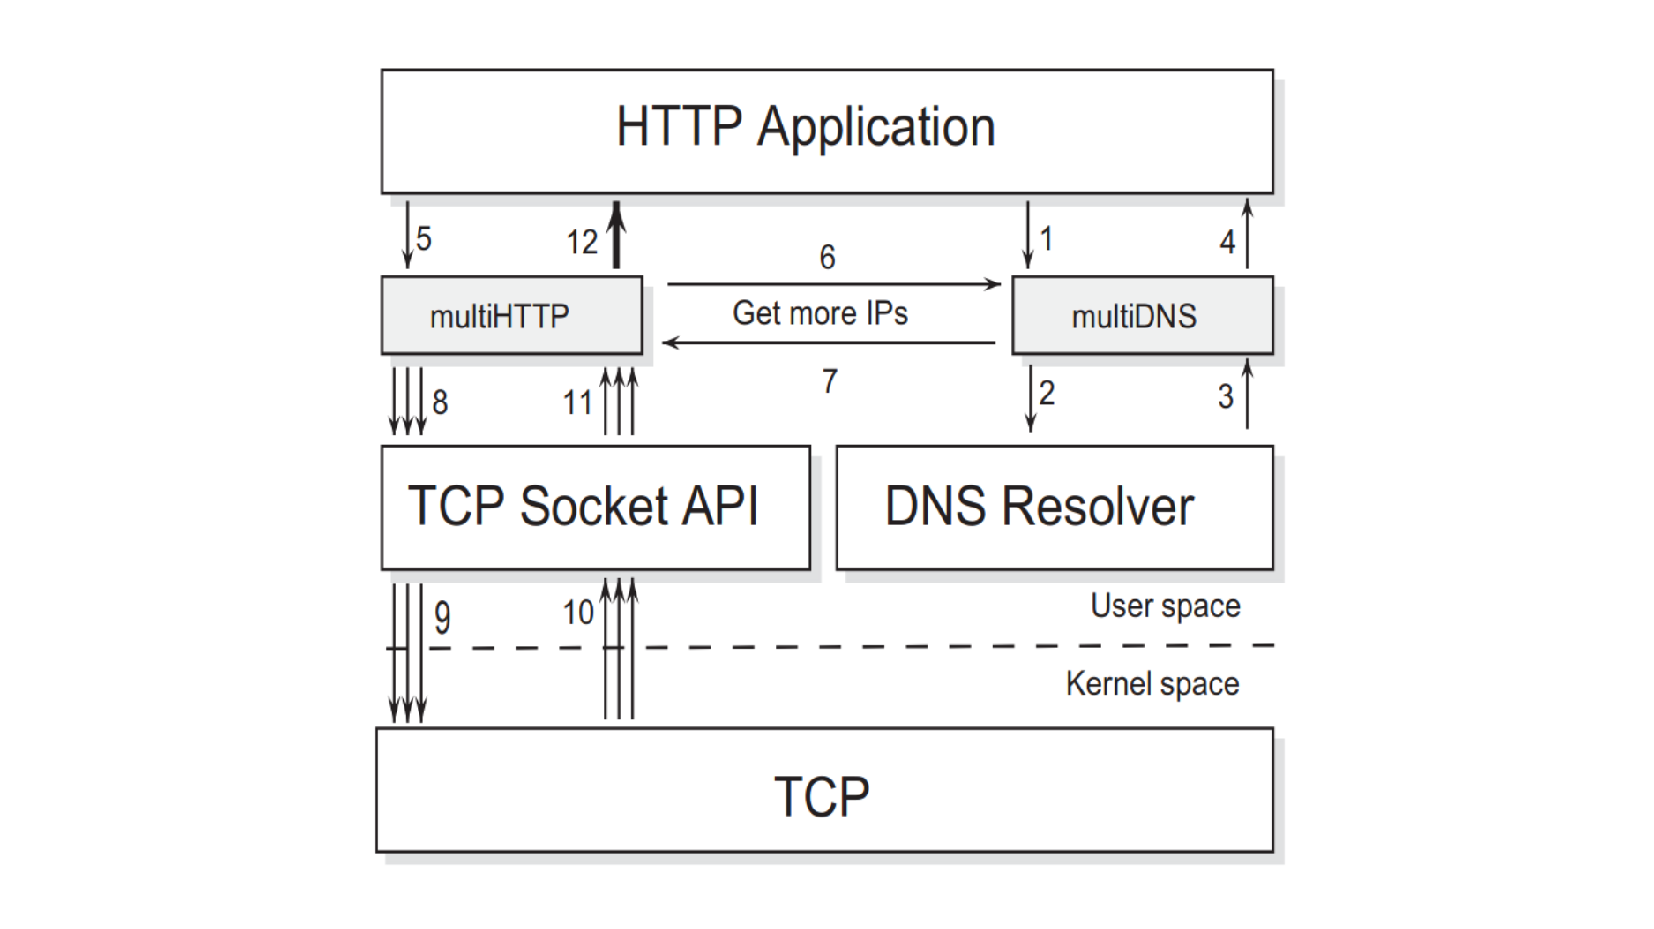
\includegraphics[width=16cm]{figure/mhttp.pdf}
	\caption{mHTTPの構造}
	\label{mhttp}
\end{figure}

\newpage

また,複数のTCP接続を使用して,複数のサーバーから同一のファイルを取得し,クライアントに対して単一のバイトストリームとして応答を返すHTTPプロキシの提案が既になされている.\cite{proxy}
この研究では遅延しているブロックに対する冗長的な重複再要求を行うことで,バッファの使用量の削減とスムーズなダウンロードを実現しながらも,冗長な要求によるダウンロード時間の増加を抑える試みが提案されている.


\section{プログレッシブダウンロード方式}
ネットワークの大容量化,高速化に伴い,Youtube\cite{youtube}やNetflix\cite{netflix}などの動画配信サービスの利用が増加している.
動画配信サービスにはUDP上に独自のアプリケーションプロトコルをサーバーおよびクライントに実装し利て配信するプッシュベースの方式と,TCP上でHTTPを用いて利用するプルベースの方式などがある.
中でもアプリケーションプロトコルとしてHTTPを用いるプルベース方式は,エンドユーザーは特別なソフトウェアの準備等をする必要はなく,基本的にはブラウザさえあれば利用可であり,またアプリケーションプロトコルがHTTPであることからサービスの提供者もAkamaiやFastlyに代表されるCDNのサービスを利用することで効率の良い配信が可能であるため,近年急速に広がっている.
HTTPを利用したストリーミング方式としてはHLS(HTTP LiveStreaming)\cite{hls}やMPEG-DASH(MPEG-Dynamic Adaptive Streaming over HTTP)\cite{dash}がある.
プログレッシブダウンロードとは,こうしたプルベース方式の中でも基本的なファイルのダウンロードを応用することでファイルを部分的にダウンロードしながらダウンロードの完了した部分からブラウザのレンダリングや動画再生等に利用する方式である.\\
\ \ \ \ プログレッシブダウンロードでは基本的にはダウンロード済みのデータはキャッシュとして再利用可能であるので,著作権など再利用に制限を加えたい場合や生放送形式での動画配信についてはをHLSやMPEG-DASHベースとしてフロントエンドおよびサーバーサイドでの実装が必要である.
プログレッシブダウンロードの動作概要は,まず,1つのファイルを複数のあるサイズのブロックに分割する.
次に,クライアントは分割されたブロックをサーバーに対してリクエストする.
サーバーはリクエストに応じたブロックを送信する.
これを繰り返すことで,1つのファイルを取得できる.
このリクエストの方法の1つにHTTPのRange-Headerに分割のための情報を含める方式がある.
この方式はRange-Headerに対応したHTTPサーバーがあれば利用が可能である.
他にもHTTPのGETリクエストのクエリストリングに分割のための情報を含める方式や,HLSやMPEG-DASH等で用いられている事前にファイル情報が書き込まれたファイルを取得し,分割済みのファイルの一部をリクエストする方式などがある.

\begin{figure}[h]
	\centering
	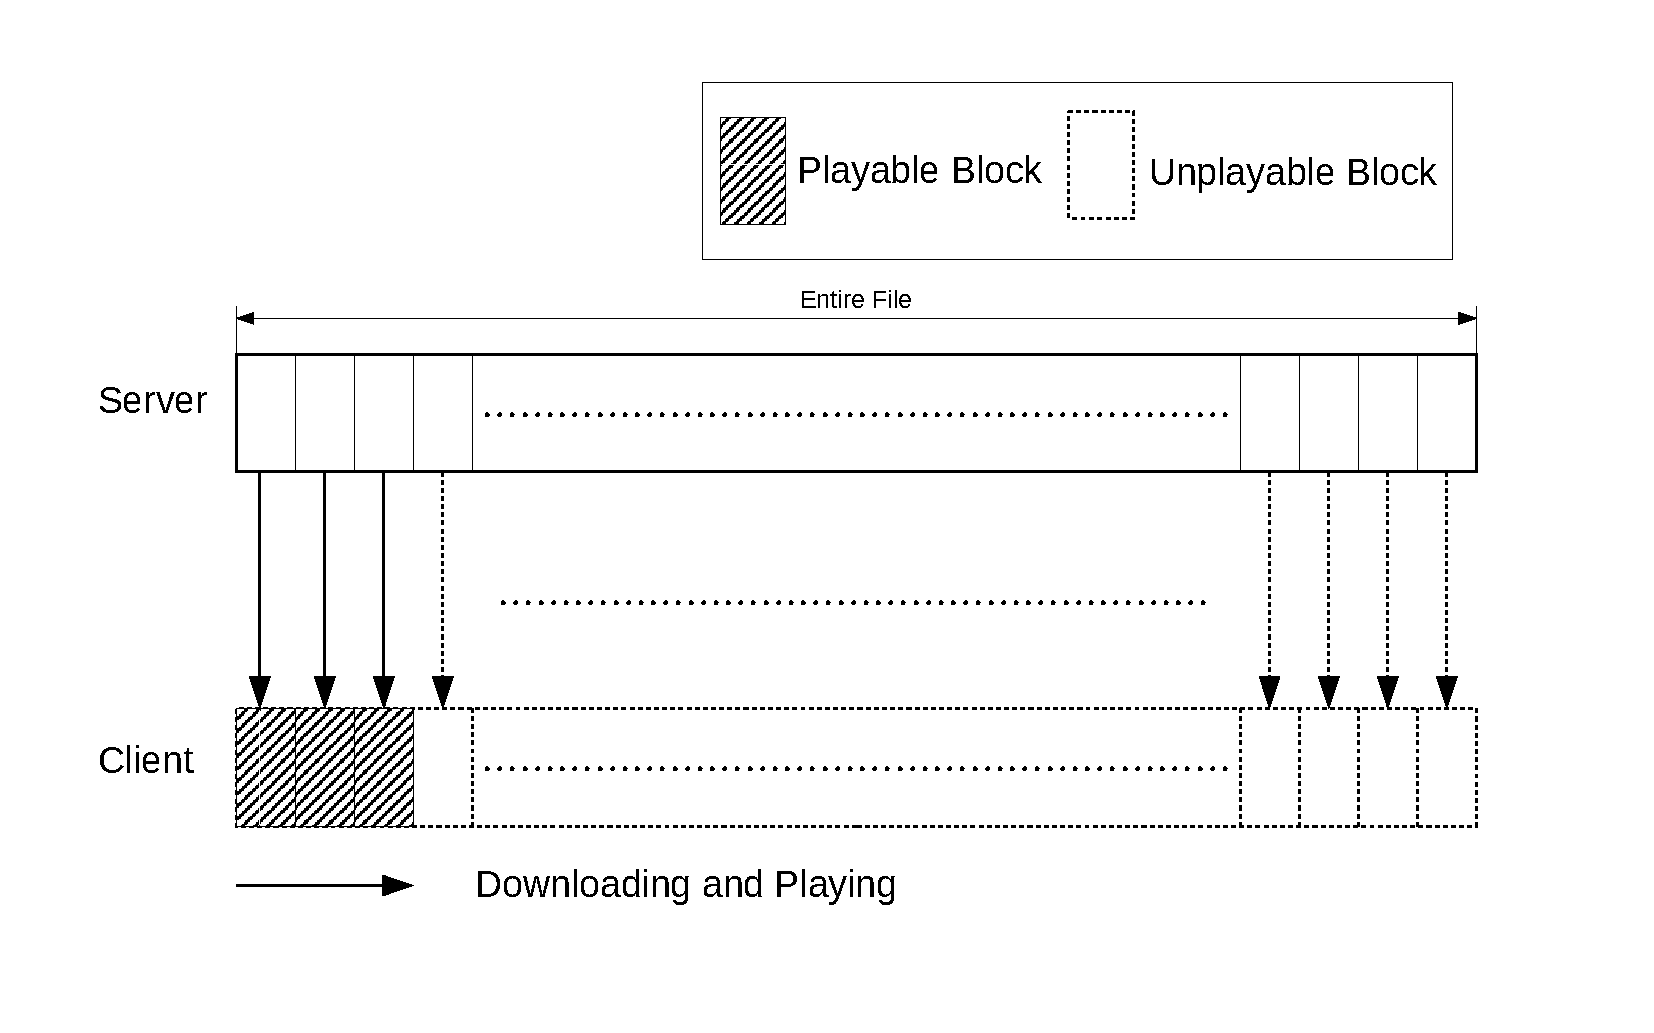
\includegraphics[width=16cm]{figure/p-dl.pdf}
	\caption{プログレッシブダウンロードの模式図}
	\label{p-dl}
\end{figure}

\clearpage

\section{複数TCP接続を用いたプログレッシブダウンロード}
\label{hukusu}
ネットワークの発展に伴い,大容量のデータをTCPを用いて,通信する機会が増加しつつある.TCPには輻輳回避のためにウィンドウ制御が存在する.
このため,ウィンドウサイズを遅延で割ったものが単一TCP接続における理論最大性能となる.
近年ではコンテンツの大容量化が進んでおり,より効率よくコンテンツをダウンロードするためにアプリケーション層から複数のTCP接続を用いる手法が提案されている.
図\ref{block}は複数のTCPを接続を用いたプログレッシブダウンロードの分割されたブロックの受信の様子を示した例である.
複数のブロックを性能の異なる別々のTCP接続に対して要求を行う場合,ブロックの再生順番と受信完了順序が一致しない可能性がある.
図\ref{block}が示すように,先頭から連続するブロック1及びブロック2は再生可能である(有効ブロック)が,それ以外のブロック3及びブロック5は未受信のブロックを間に挟んでいるため再生することはできない(非有効ブロック).
複数のTCP接続を束ねることでグッドプットを向上させても,受信ブロックが有効ブロックでない限りは応答性は低下してしまい,動画の再生が停止するなどしてユーザー体験は悪化することが予想できる.
また,バッファ使用量の観点から見ても多数の非有効ブロックをメモリ上に保持し続けるのは,好ましくないと言える.
先行研究では帯域の有効活用を目と機としてホストとの間に複数のTCP接続を確立する手法が提案されている\cite{hiraoka}.

\begin{figure}[h]
	\centering
	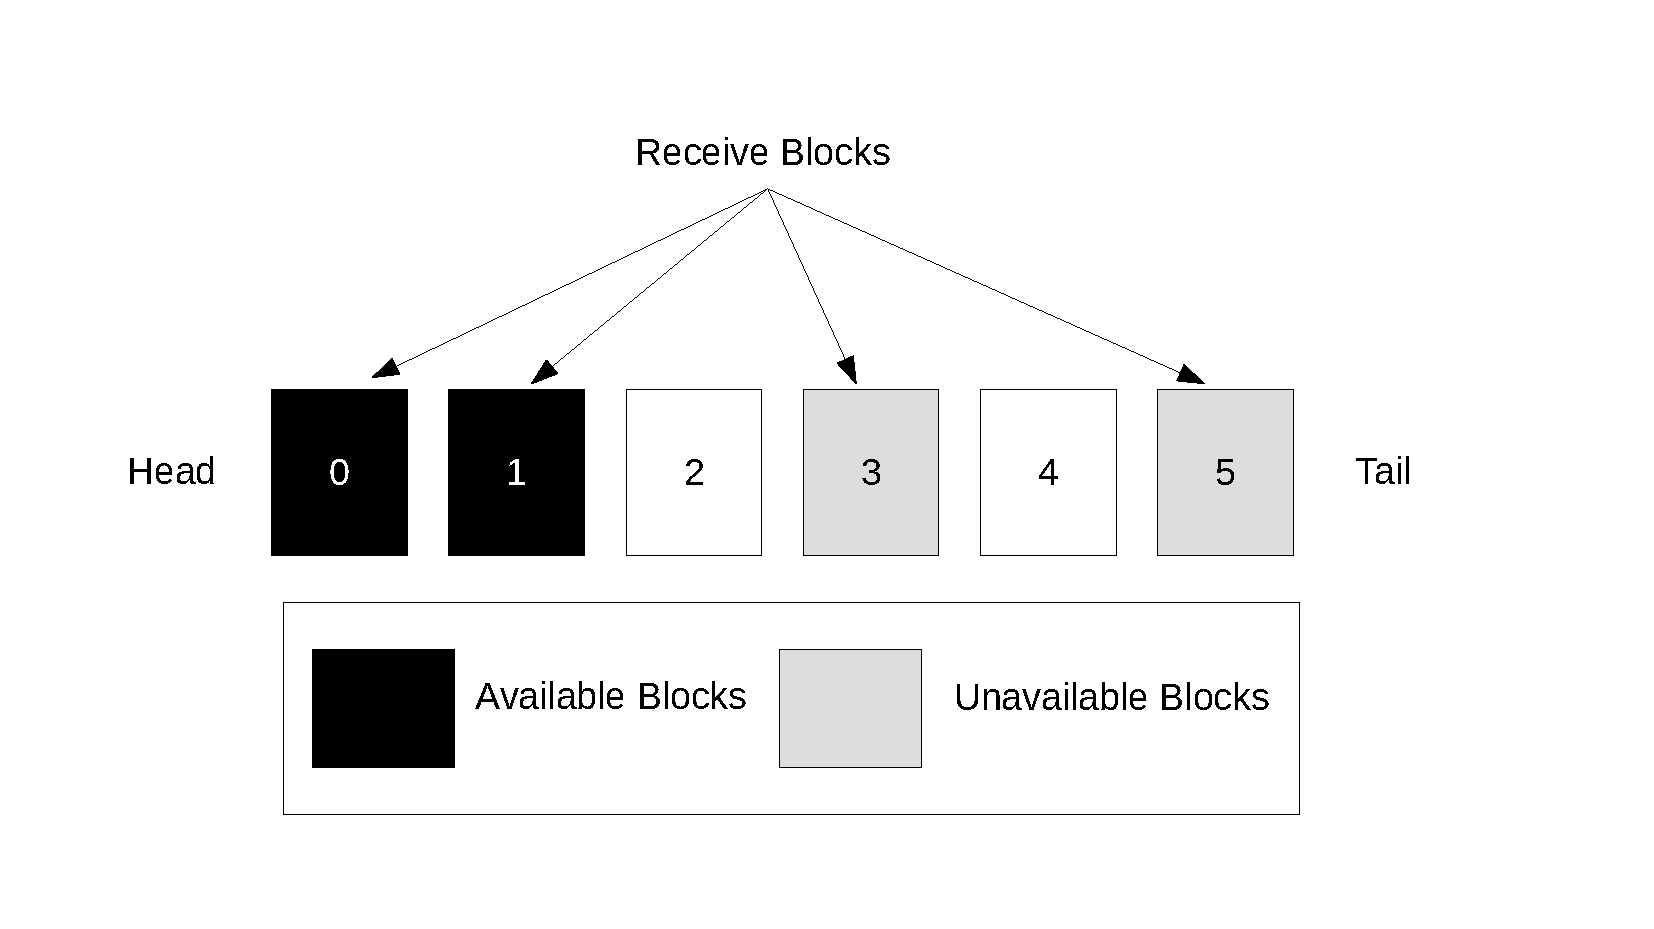
\includegraphics[width=17cm]{figure/block.pdf}
	\caption{ブロックの有効性}
	\label{block}
\end{figure}

 %%%%%%%%%%%%%
 \section{重複再要求}
 \label{juhuku}
 \ref{hukusu}節で述べた性能差のある複数のTCP接続を用いたプログレッシブダウンロードにおいて起こりうる問題点を,アプリケーション層での制御で解消するための重複再要求方式が関連研究\cite{proxy}において提案されている.
 この方式では未取得ブロックより後に合計N個以上(有効・非有効は問わない)のブロックがあれば,未取得ブロックをその未取得ブロックを要求したTCP接続とは別のTCP接続へ再要求を行う.
 図\ref{blockdup}にその模式図を示す.
 図\ref{blockdup}の例では重複再要求を行い,ブロック2を取得することで少なくともでもブロック3が非有効ブロックである状態を解消することができる.
 この操作を受信イベントが発生するたびに繰り返すことで,バッファ上の非有効ブロックの個数の増加を抑制することができ,応答性の向上が見込まれる.
 
 \begin{figure}[ht]
     \centering
     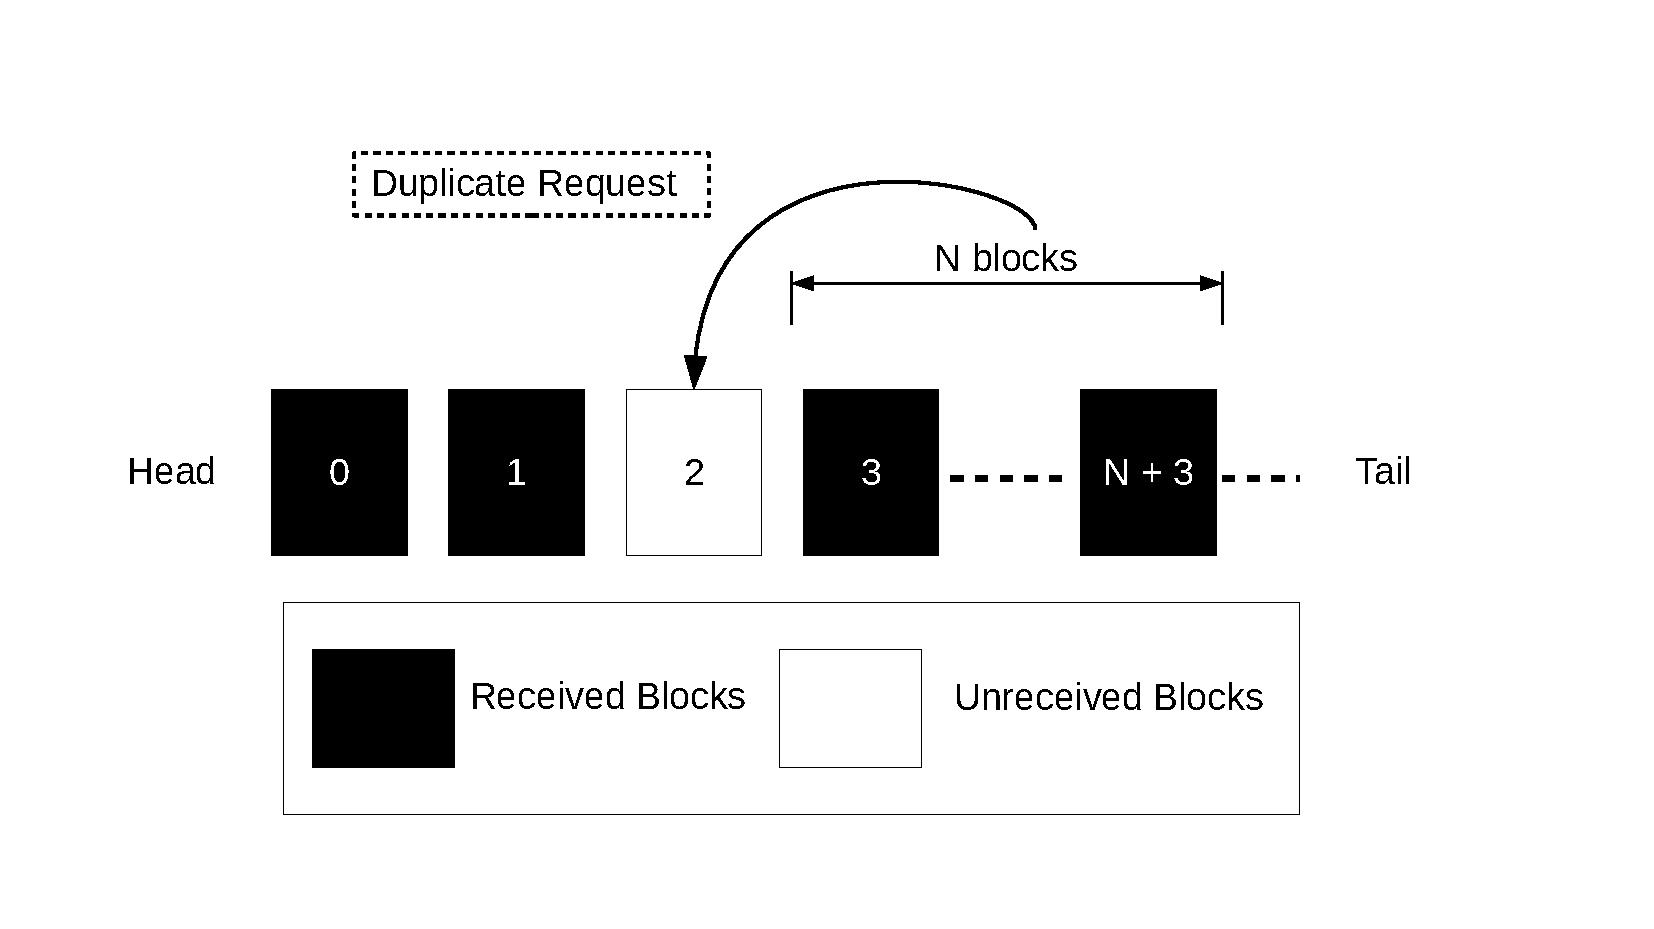
\includegraphics[width=18cm]{figure/block_dup.pdf}
     \caption{重複再要求の模式図}
     \label{blockdup}
 \end{figure}

\newpage
 
\section{タイマ駆動を用いた要求方式}
\ref{hukusu}節で述べた複数のTCP接続を用いたプログレッシブダウンロードにおいて起こりうる問題点を解消するために提案されている方式として,タイマ駆動型要求方式がある\cite{horiba}.
\ref{juhuku}節で述べた重複再要求方式は,ブロックの遅延に対して後から対処するという方針である.
重複再要求を行うことは帯域の冗長的な利用であるので,
そもそもの非有効ブロックの受信を減らすための制御も必要であると言える.
本節で述べるタイマ駆動を用いた要求方式は,TCP接続の性能差を予め考慮することで,到着順序逆転の発生そのものを抑制しようという方針である.
はじめに比較対象となる受信駆動を用いた要求方式について説明する.
受信駆動とは,あるTCP接続に対して常時1つのブロックを要求する方式である。
ブロックの受信が終了したら次ブロックに対する要求を送信する.
タイマ駆動とは前ブロックの要求送信からある時間が経過したら次ブロックへの要求を行う.
このとき前ブロックの受信完了を待つことはない.
図\ref{timer}に模式図を示す.

先行研究としてはタイマ駆動を用いた要求方式において,TCP接続間の性能差を要求の送信間隔に反映させる方式が提案されている.

 \begin{figure}[ht]
 	\centering
 	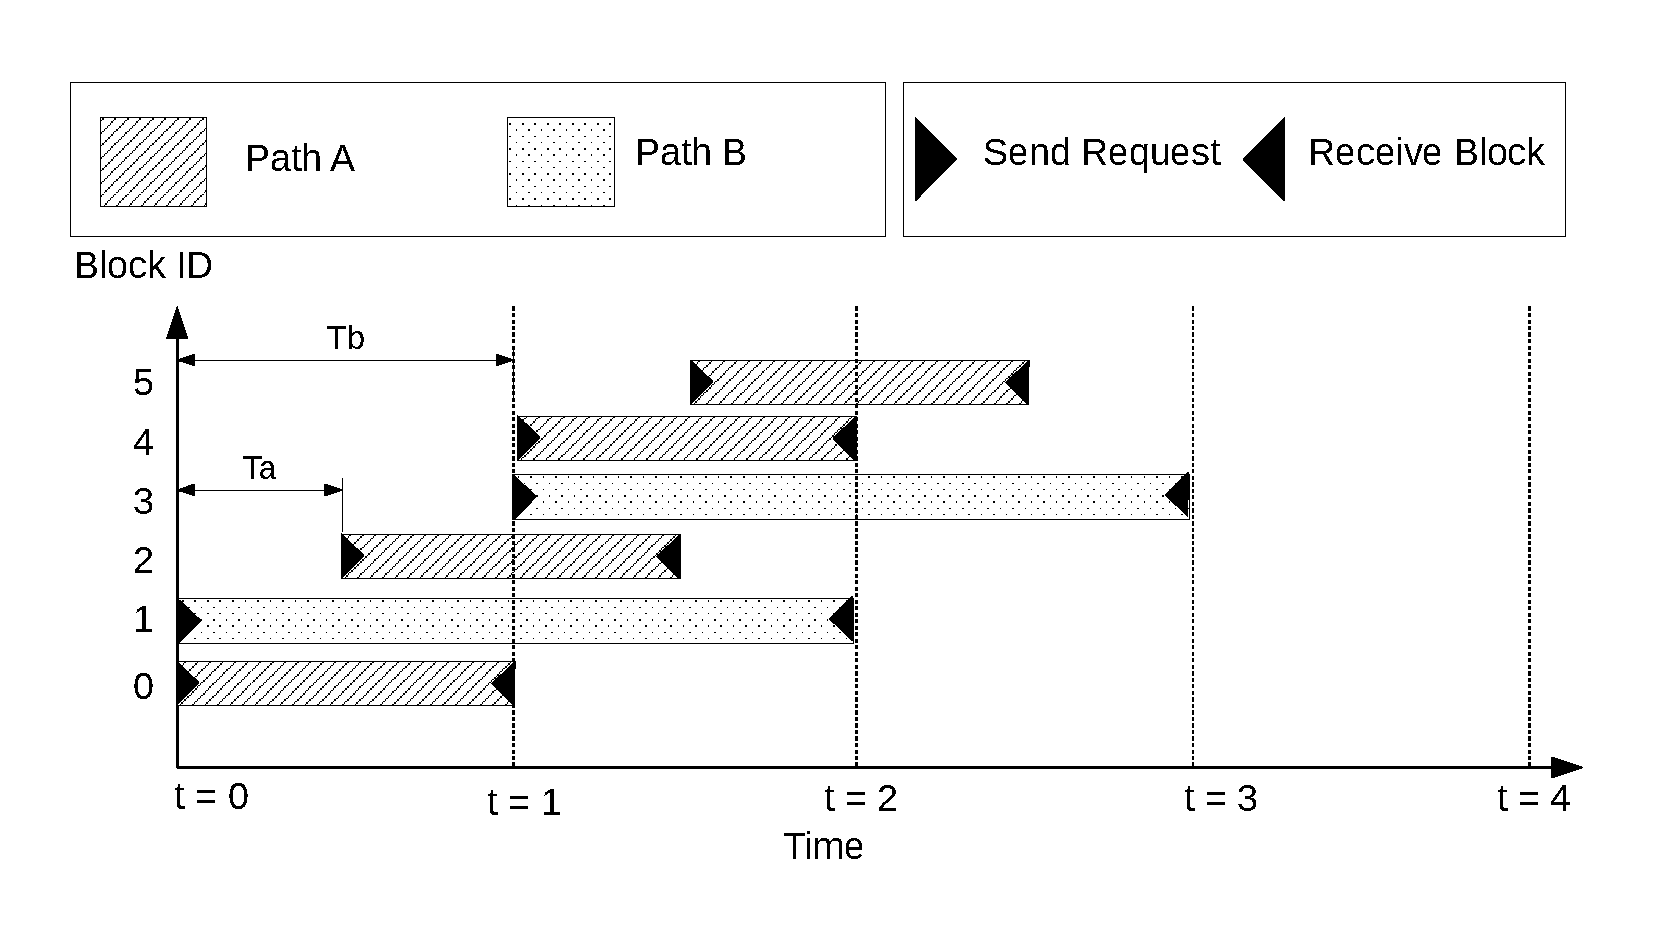
\includegraphics[width=16.5cm]{figure/timer.pdf}
 	\caption{タイマ駆動方式の模式図}
	\label{timer}
 \end{figure}
 
\chapter{提案方式}\label{sec:sec3}
本章では性能差のある複数のTCP接続を並列的に利用する際に生じうるいくつかの問題点を解消するためのアルゴリズムを実装した提案方式について述べる.
また,実際に複数のTCP接続を用いた動画のプログレッシブダウンロードをプログラムに実装する際に考慮すべき点がいくつかある.
動画のプログレッシブダウンロードの実装は大きく分けて動画ファイルのダウンロードとバイナリをデコードして再生という2つのセクションに分かれている.
既存のウェブブラウザやVLC\cite{vlc}等のネットワークメディア再生機能付きの動画プレイヤーソフトのではこの2つのセクションは1つのプログラムから高度に同期をとりながら同時並列的に制御されている.
しかし,本研究では実装の難易度の高さ,主としてダウンロードセクションについて論じるため,そして公開ネットワーク上での評価を行うためにこれら2つのセクションのうちダウンロードセクションのみを対象とする.

\section{遅延要求方式}
\label{chienyokyuhoshiki}
\ref{chienyokyu}節では遅延要求の概要について述べる.
\ref{kotei}節では各接続の帯域が既知であるいう仮定に基づいて,TCP接続の性能差を入力し,ブロックの要求位置を変化させることで到着順序逆転の抑制する方式について提案する.
\ref{diff}節では未知のネットワーク状況に対応するためにTCP接続の使用回数の差分に注目しブロックの遅延度を推測する方式について提案する.
また,本研究では各TCP接続には同時に最大でも1つのHTTP リクエスト-レスポンスしか発行しない.
つまりタイマ駆動方式など用いられているHTTP-パイプラインは用いず,受信駆動モデルで実装を行う.

\newpage

\subsection{遅延要求について}
\label{chienyokyu}
この章で定義する遅延要求についての概要を述べる.まず,確立したTCP接続群の中で性能の最も高いTCP接続には,要求が未送信である最も若番のブロックを要求する.
ここでの最高性能の定義は使用回数が最多の接続とする.
比較性能の低いあるTCP接続には,その時点での最も若番ではないブロックを要求する.
以降,この最も若番ではないブロックを要求することを遅延要求と呼称する.
遅延要求を行うことで,非有効ブロックの受信を頻度が減少するので,
結果として重複再要求における冗長な帯域使用も抑制することができる.

図\ref{delay}にその模式図を示す.
この例では,接続Aは接続Bの2倍の性能を持ち,接続Aは最高性能であると仮定する.
まず,この条件より接続Bがブロックを1個取得する間に接続Aはブロックを2個取得取得することが予想でき,
接続Bは最若番よりも2つ後ろのブロックを要求する.
\begin{math}t=0\end{math}において,
最高性能である接続Aには最若番のであるブロック0を,
接続Bには2つ後ろであるブロック2を要求する.
これを繰り返すことで図\ref{delay}の例ではブロック0-5が順序逆転を起こすことなく,
順序通りに到着する.

\ref{kotei}節ではあらかじめ各接続間の性能差が既知であるとして,その値にしたがって遅延要求を行う方式について述べる.
\ref{diff}節では各接続ごとにブロック到着間隔を逐次測定することで性能差を算出し,その値にしたがって遅延要求を行う方式について述べる.

\begin{figure}[ht]
    \centering
    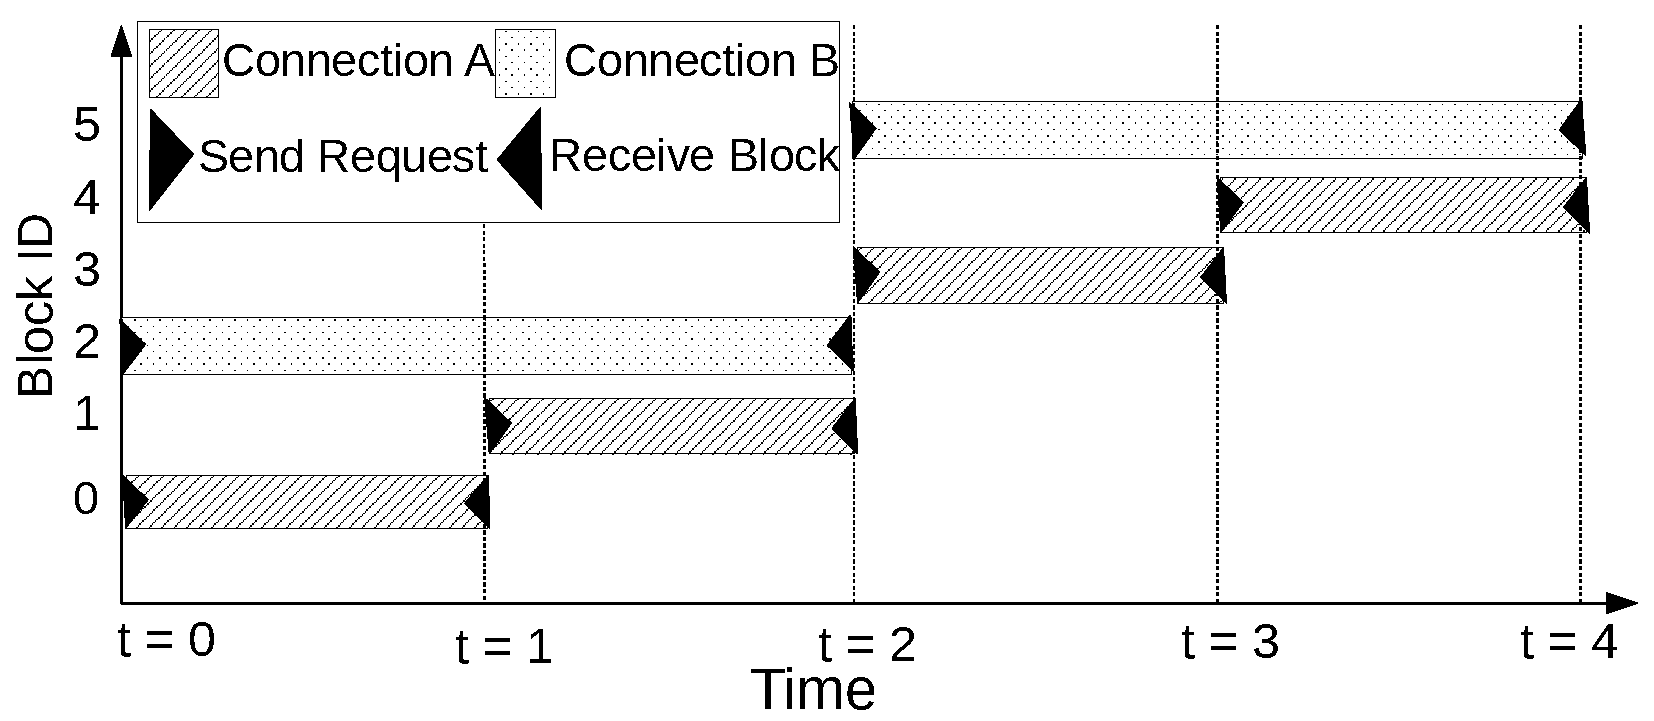
\includegraphics[width=16.25cm]{figure/delay-n.pdf}
    \caption{遅延要求の模式図}
    \label{delay}
\end{figure}

\subsection{固定遅延要求方式}
\label{kotei}
固定遅延方式は,予めTCP接続間の性能差をシステムに入力して遅延要求を行うことで到着順序逆転の抑制を試みる方式である.
しかし,実ネットワークでは予めTCP接続間の性能差が既知であることは稀であるので実環境への応用は限定的であると言わざるを得ない.
よって本研究では本方式は主として,他の方式がどれだけTCP接続間の性能差を正確に把握できているかどうかを比較し確認するために用いる.
詳細な動作については,\ref{chienyokyu}で述べたとおりである.

\subsection{差分計測を用いた遅延予測方式}
\label{diff}
当方式はあるTCP接続に対して何ブロック後ろのブロックを要求するかを算出するために,そのTCP接続の直前のブロック取得間隔を計測し用いる方式である.
以下に疑似コードを示す.
最も性能の高いTCP接続には最も若番として0を割り当てる.

\begin{algorithm}
	\caption{Compute Diff}
	\begin{algorithmic}[1]
		\State {$T \gets Total\ Receive\ Count$}
		\State {$P[X] \gets Previous\ Total\ Receive\ Count\ for\ Connection\ X$}
		\State {$N \gets Number\ Of\ Connections$}
		\If{Is \begin{math}X\end{math} the highest performance} 
		\State {$D \leftarrow 0$}
		\Else 
		\State {$D \leftarrow T - P[X] - N + 1$}
		\EndIf
	\end{algorithmic}
\end{algorithm}

このアルゴリズムでは一つ前の送信時から現在まで全体の総受信ブロック数のカウントがいくつ増加したかを計算する.
なお,このアルゴリズムではTCP接続の性能の時間変化については考慮していない.
よってTCP接続に急激な性能変化が発生した場合などに予測的な見積もりを行うことはできないので,追従が遅れる可能性がある.

\newpage

\section{初期遅延予測}
\label{shoki}
\ref{diff}節の遅延要求方式は実装上の都合,このままでは最初のリクエスト送信の際にはTCP接続間の性能差が不明であるため,遅延要求を行うことができない.
よって性能の低い接続に要求した初期ブロックが遅延すると,動画再生開始時に待ち時間が生じる可能性がある.
しかし実際にエンドユーザーが動画再生を行うことを想定すると,再生開始時における待ち時間の長さは視聴体験に大きく影響を及ぼすことが予想される.
本節ではこの問題の解決案として初期値を予測し初期バッファリング時間の短縮を目指す方式を提案する.

\subsection{概要}
\label{shokigaiyo}
\ref{chienyokyuhoshiki}節の遅延要求方式では,事前にHTTPのHEADリクエストを相手サーバーに送信し,ファイルサイズ等の情報を取得する.
このHEADリクエスト-レスポンスの応答時間を計測することで,各TCP接続間の性能差も推測できる.
ただし,後続のGETリクエストの応答メッセージサイズはHEADリクエストのそれよりも大きく,実際には一つのHTTPレスポンスに対して複数のTCPセグメントがやり取りされるので,厳密な意味での応答時間ではなく単一のHEADリクエスト-レスポンスの応答時間であることに注意が必要である.
\begin{math}D(a), D(b)\end{math}間の比から\begin{math}T(a), T(b)\end{math}間の比を予測することが初期遅延予測の目的である.
図\ref{head}に初期遅延予測の模式図を示す.

\begin{figure}[ht]
	\centering
	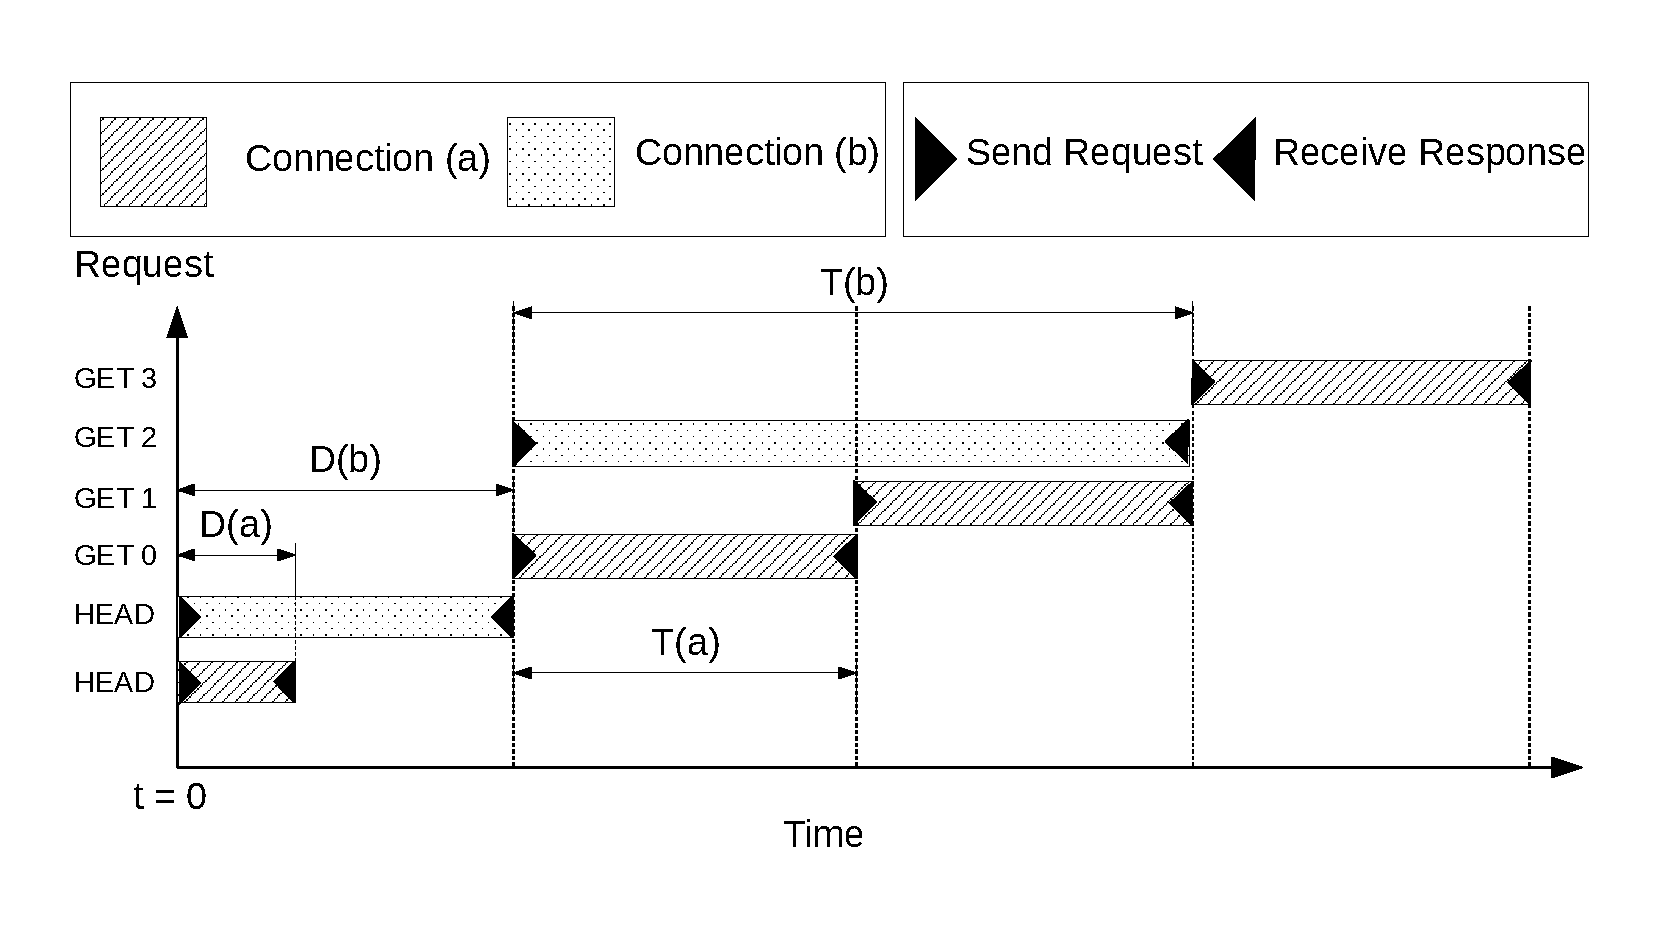
\includegraphics[width=14cm]{figure/head.pdf}
	\caption{初期遅延予測の模式図}
	\label{head}
\end{figure}

\newpage

\subsection{アルゴリズム}
\label{yosokuhouhou}
本節では具体的な初期遅延予測アルゴリズムについて述べる.

\subsubsection{初期遅延予測係数}
ここで定義する遅延予測係数とは,各TCP接続でのHTTP HEAD リクエストの応答時間の比をTCP接続の帯域性能差へ変換するための係数である.
TCPのウィンドウサイズがネットワーク状況に応じて変化することや高遅延でありながらも広帯域のネットワークが実際に存在することを考慮すると,初期応答時間からTCP接続の性能を単純に予測することは現実的ではない.
しかし,仮に広帯域であっても高遅延なネットワークではTCPのウィンドウサイズが大きくなるまでに低遅延ネットワークよりも長い時間がかかる.
また,初期ブロックの到着時刻がユーザー体験に与える影響は大きいと考えられる.
よって初期リクエストの送信時に限って言えば,多少の性能予測が外れることは許容しても,低性能の可能性がある高遅延なTCP接続にはとにかく初期ブロックを要求させないことが,初期バッファリング時間の短縮につながる.
各接続における初期リクエスト-レスポンスさえ終了してしまえば,そこからは性能計測は差分予測の役割になる.
つまり,応答遅延時間から最悪ケースとして冗長的にTCP接続の性能を見積もることで,ユーザー体験の悪化を防ぐことが目的である.

\subsubsection{算出}
初期遅延度は各TCP接続において計測したHEAD リクエストの応答時間と,すべてのTCP接続の応答時間の最小値との比に初期遅延予測係数を掛けることで算出する.
以下に疑似コードを示す.

\begin{algorithm}
	\caption{Compute Initial Delays}
	\begin{algorithmic}[1]
		\State {$R \gets Raw\ Delays $}
		\State {$M \gets MIN(R)$}
		\State {$D \gets Delays $}
		\State {$C \gets Coefficient$}
		\ForAll {r in R}
		\State {$d \leftarrow (r \ / \  M - 1) \ * \ C$}
		\State {$Add\ d\ to\ D$}
		\EndFor
	\end{algorithmic}
	
\end{algorithm}


\chapter{実装評価}\label{sec:sec4}

本章では提案方式を実装し,評価する.

\section{提案手法の実装}
提案手法を実装したプログラムの概要を説明する.
実装はPythonで行った.
まず,ユーザーは複数のホストのURL,分割サイズ等を引数とするオブジェクトを生成する.
プログラムはURLが有効であるかをHTTP HEADリクエストを用いて確認する.
入力された分割サイズを元にブロック1個あたりのバイト数を決定し,
HTTP-Range リクエストに必要なヘッダーを生成してスレッドセーフなキューに保管する.
便宜上キューと呼称しているが、
このキューは任意の位置のデータを取り出すことのできるように改良してある.
次にホストとの接続を確立する.
ここでは既存のHTTPライブラリをセッション層に利用している.
ここまでがコンストラクタである.
ユーザーがダウンロード開始メソッドを呼び出すと,ホスト数だけの子スレッドを起動する.
各子スレッドはファイル全体が揃うまでキューからヘッダーをとりだして各ホストに要求を送信し,
ブロックの受信が終了したらスレッド共有のメモリ上に保管したのち親スレッドに通知を送信するという作業を繰り返す.
親スレッドはユーザーからのデータの読み出しがあった場合,共有メモリを確認してその時点で順序が揃った部分を連結してユーザーに返却する.
このときユーザーに返却すべきデータが存在しない場合,子スレッドからの通知を待つ.
この返却についてはイテレータを利用することで,
ユーザーは任意のタイミングで順序の揃った部分を読み出すことができる.
図\ref{sphttp}に提案手法についての概要を示す.

%\clearpage

\begin{figure}[h]
	\label{sphttp}
	\begin{center}
		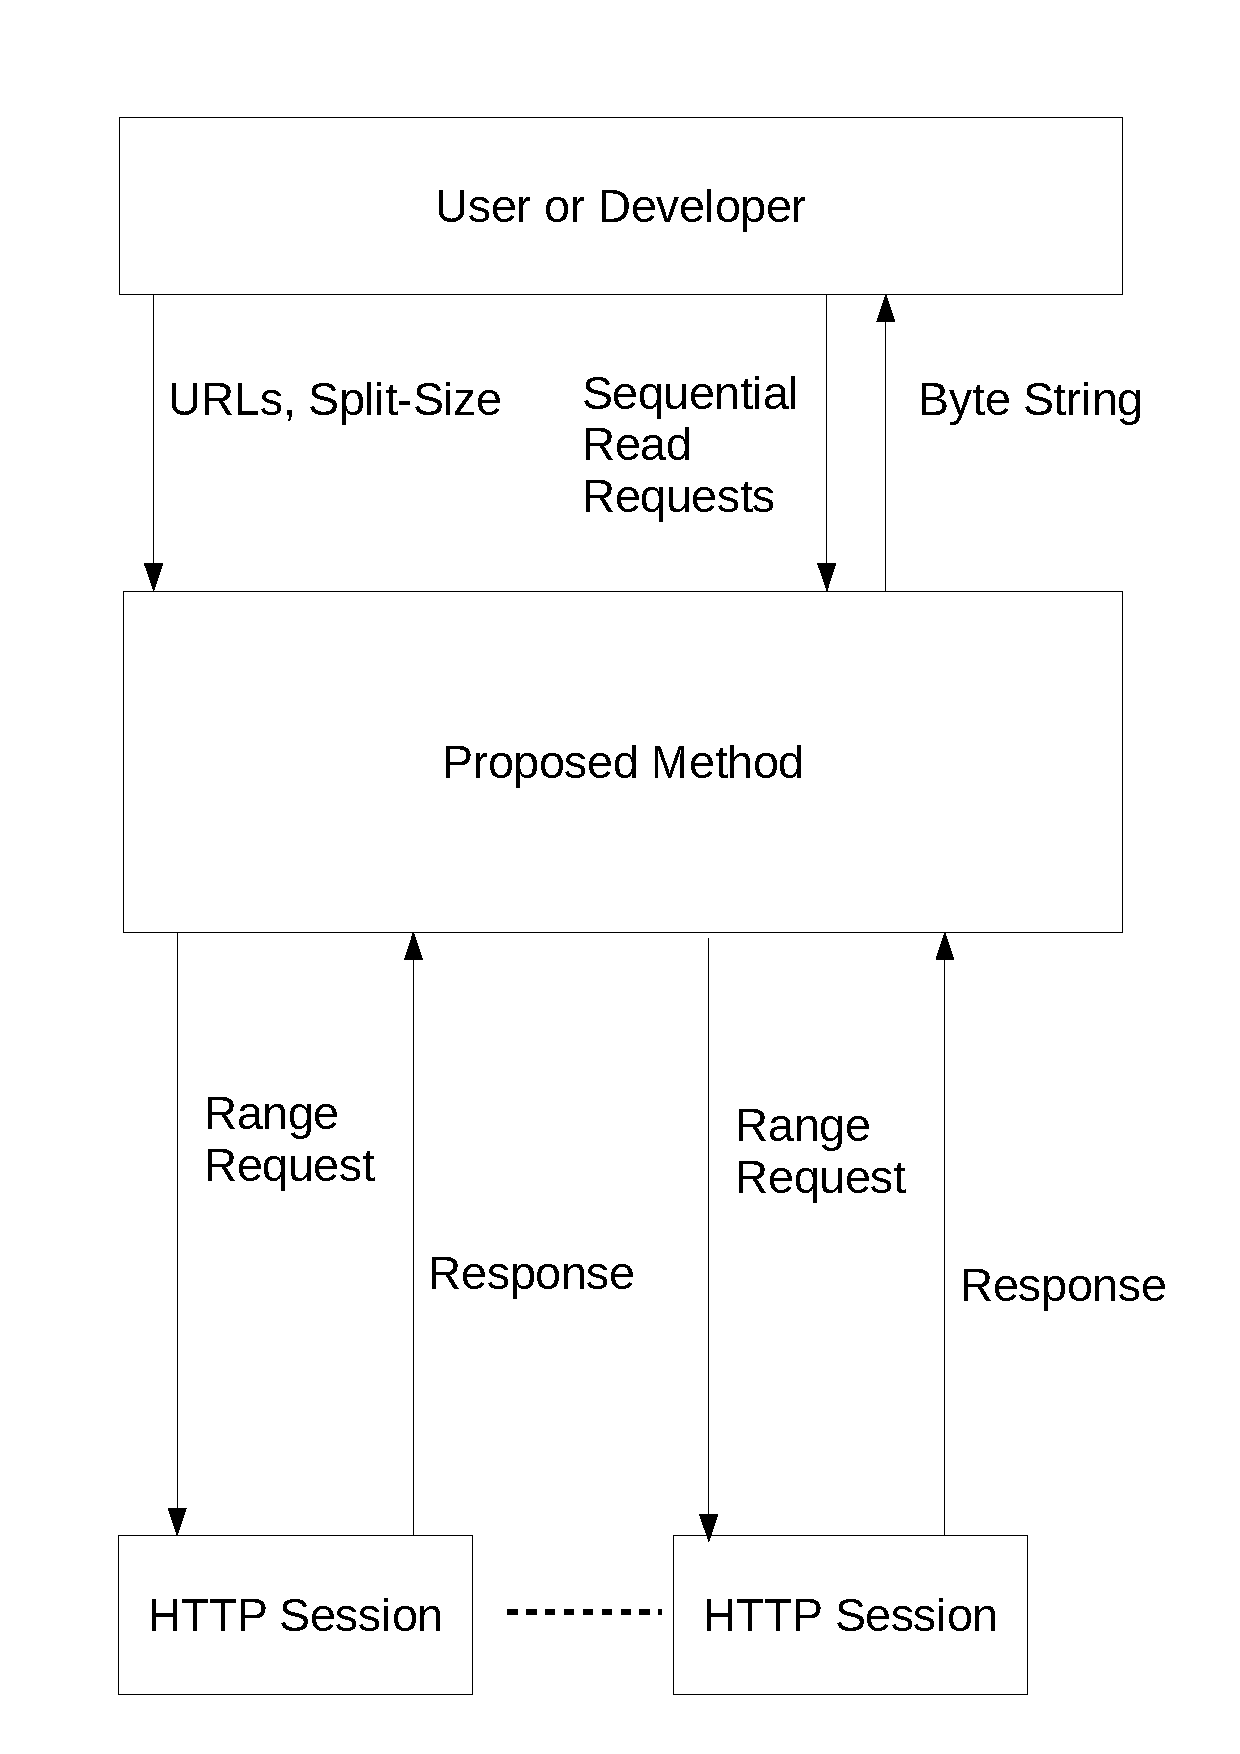
\includegraphics[width=15cm]{figure/sphttp.pdf}
		\caption{提案手法についての図}
	\end{center}
\end{figure}

\clearpage


\section{評価対象}
本評価では重複再要求方式として\ref{juhuku}を改良し非有効ブロックの受信回数を閾値として用いる.
これは実装上の都合であり,関連研究のアルゴリズムとは若干異なるが本研究では重複再要求の実装方式を比較することは目的としない.
既に重複再要求方式の有効性は先行研究において確認されているので,全ての実験は重複再要求を行うことを前提としている.
また,取得するファイルは映像と音声合わせてビットレートが40Mbpsで長さが150秒の動画の取得を仮定し,
公開ネットワーク上でも容易に実験が可能である754MByteのUbuntuのリリースイメージファイルを選択した.

\section{評価項目}
\label{hyoukakoumoku}
本節では本章で行う実験で評価する評価値について整理する.
表\ref{hyoka}に評価項目についてまとめる.
初期バッファリング時間とは,ブロックの理想的な到達時刻からどのくらい遅れているかか表す遅延時間の最大値である.
動画再生を想定して言い換えると,獲得できたグッドプットを維持しながら停止せずに再生するために必要な再生開始時の待ち時間だと言える.
非有効ブロック数はバッファ内において,取得できたのにもかかわらず再生不可能なブロックの数である.
平均遅延時間は理想的なブロック到着時刻からの正の遅延時間の平均値である.
初期バッファリング時間と平均遅延時間についての模式図を図\ref{buf}に示す.

\newpage

\begin{table}[htb]
	\begin{center}
		\caption{評価項目}
		\label{hyoka}
		\begin{tabular}{|c|c|} \hline
			評価項目 & 概要 \\ \hline \hline
			初期バッファリング時間 & 初期バッファリングに必要な時間 \\ \hline
			平均非有効ブロック数 & バッファ内の非有効ブロックの数の平均値 \\ \hline
			平均遅延時間 & 理想的なブロック到着時刻からの遅延時間の平均値 \\ \hline
		\end{tabular}
	\end{center}
\end{table}

\begin{figure}[ht]
	\label{buf}
	\begin{center}
		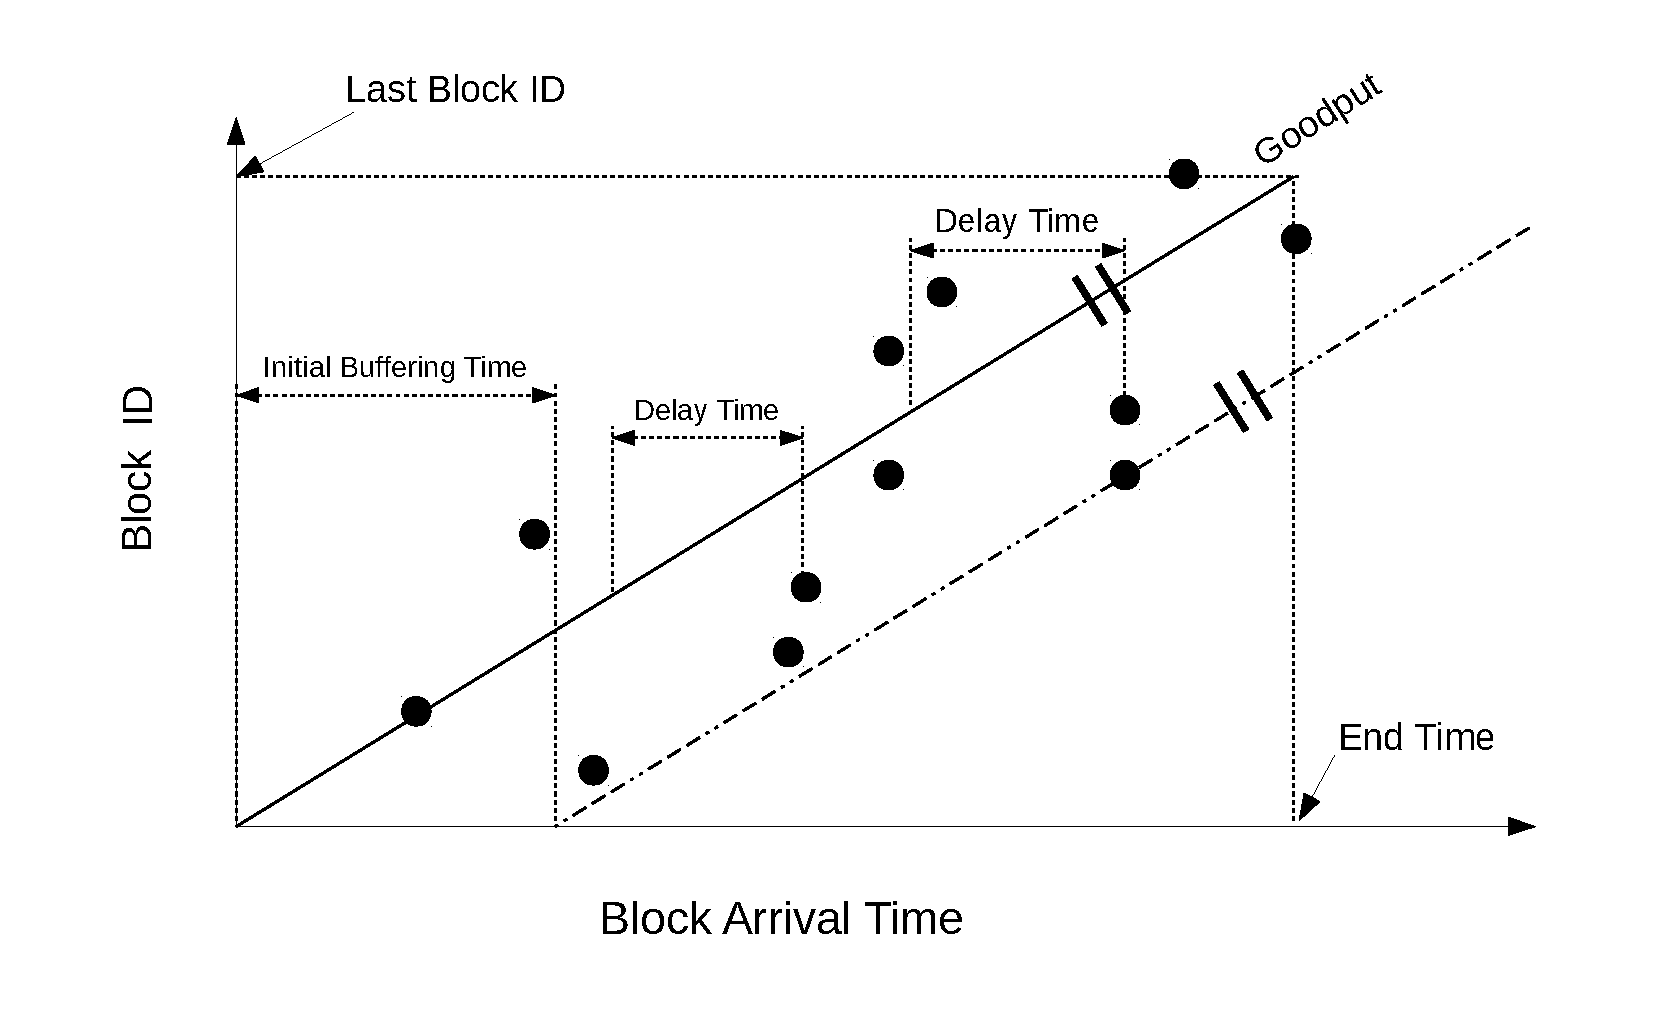
\includegraphics[width=17cm]{figure/initialBuffering.pdf}
		\caption{初期バッファリング時間と平均遅延時間の模式図}
	\end{center}
\end{figure}

\clearpage

\section{テストベッドでの評価}
\label{testbed}
\ref{networkmodel}にテストベッドのネットワーク環境を示す.
TCP接続A-TCP接続B間の性能差は3倍,TCP接続A-TCP接続C間の性能差は10倍である.
\begin{figure}[ht]
	\label{networkmodel}
	\begin{center}
		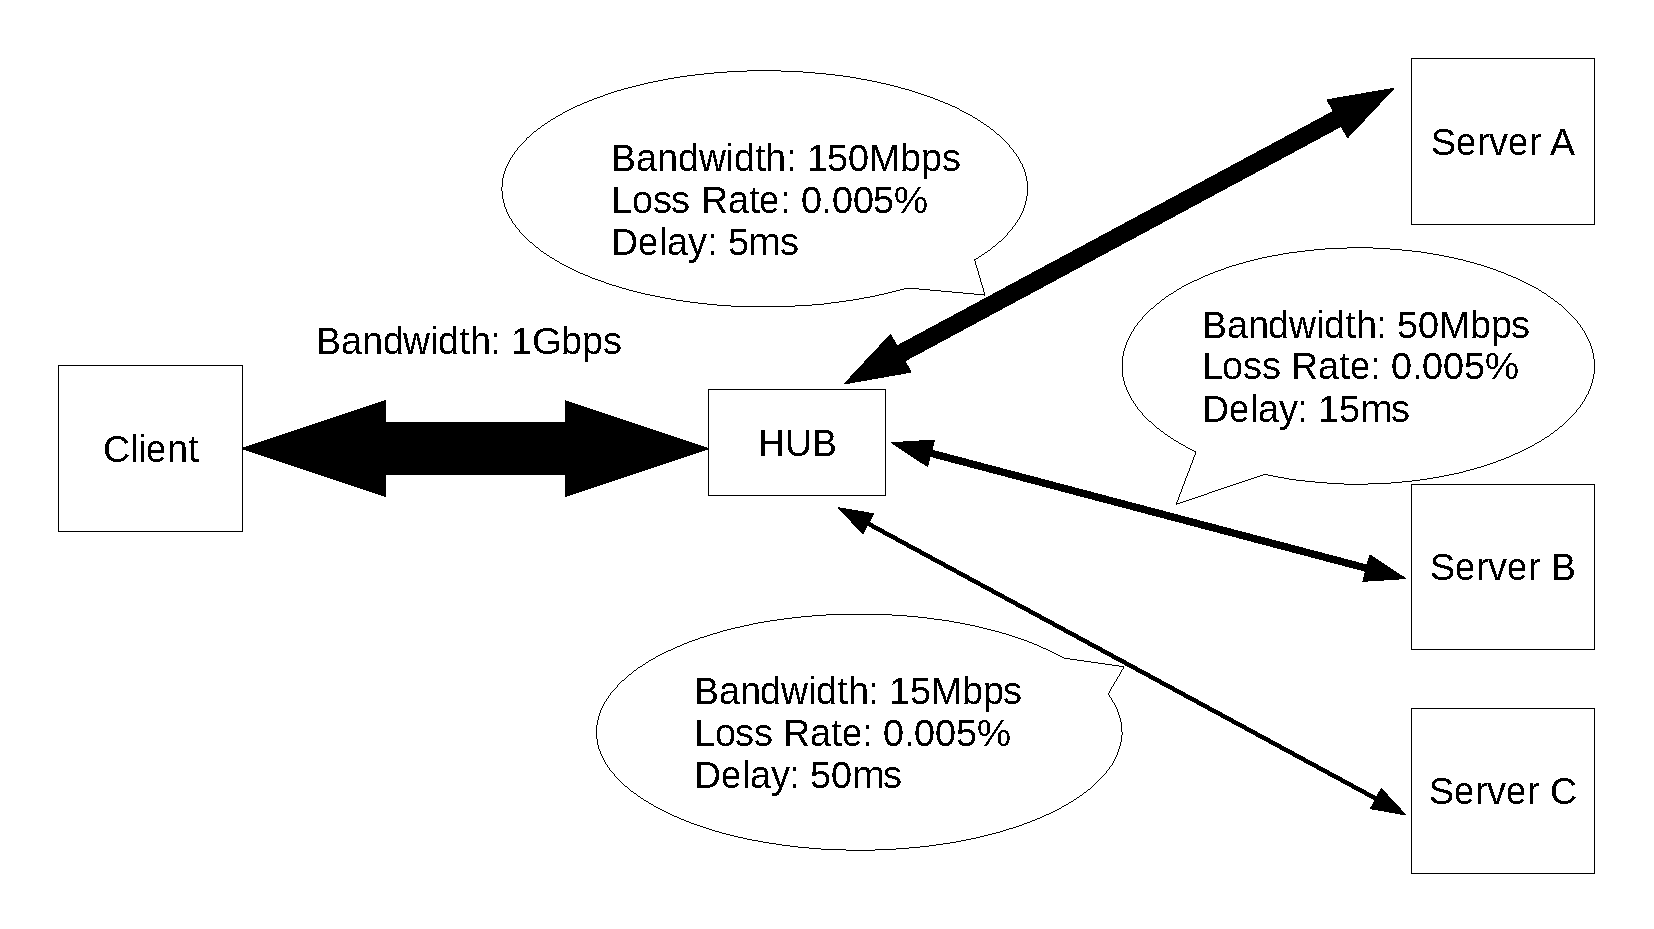
\includegraphics[width=16cm]{figure/test_network.pdf}
		\caption{ネットワーク環境}
	\end{center}
\end{figure}

実験環境および実験パラメータを表\ref{env},表\ref{param}に示す.

\begin{table}[htb]
	\begin{center}
		\caption{実験環境}
		\label{env}
		\begin{tabular}{|c|c|} \hline
			ファイルサイズ & 754MByte\\ \hline
			ファイル &  ubuntu-17.10.1-server-amd64.iso\\ \hline
			OS(Server and Client) & ubuntu 17.10 (Kernel 4.13)\\ \hline
			TCP & CUBIC \\ \hline
			HTTP Server & h2o v2.2.4 \\ \hline
		\end{tabular}
		\caption{実験パラメータ}
		\label{param}
		\begin{tabular}{|c|c|} \hline
			ブロックサイズ & \(10^6\) Byte\\ \hline
			初期遅延予測係数 & 10 \\ \hline
			重複再要求発行閾値 & 20 \\ \hline
			試行回数 & 10 \\ \hline
		\end{tabular}
	\end{center}
\end{table}

図\ref{ibt}は遅延要求のアルゴリズムごとの初期バッファリング時間である.
図\ref{nsb}は遅延要求のアルゴリズムごとの平均非有効ブロック数である.
図\ref{adt}は遅延要求のアルゴリズムごとの平均遅延時間である.
また,評価値はすべて10回試行の平均である.
DIFF-Falseは初期遅延予測を行わない差分計測を用いた遅延要求方式,DIFF-Trueは初期遅延予測を行う差分計測を用いた遅延要求方式,NORMALは常時最若番を要求する方式(重複再要求のみ),STATICはTCP接続間の性能差を入力する固定遅延要求方式である.

\begin{figure}[h]
	\centering
	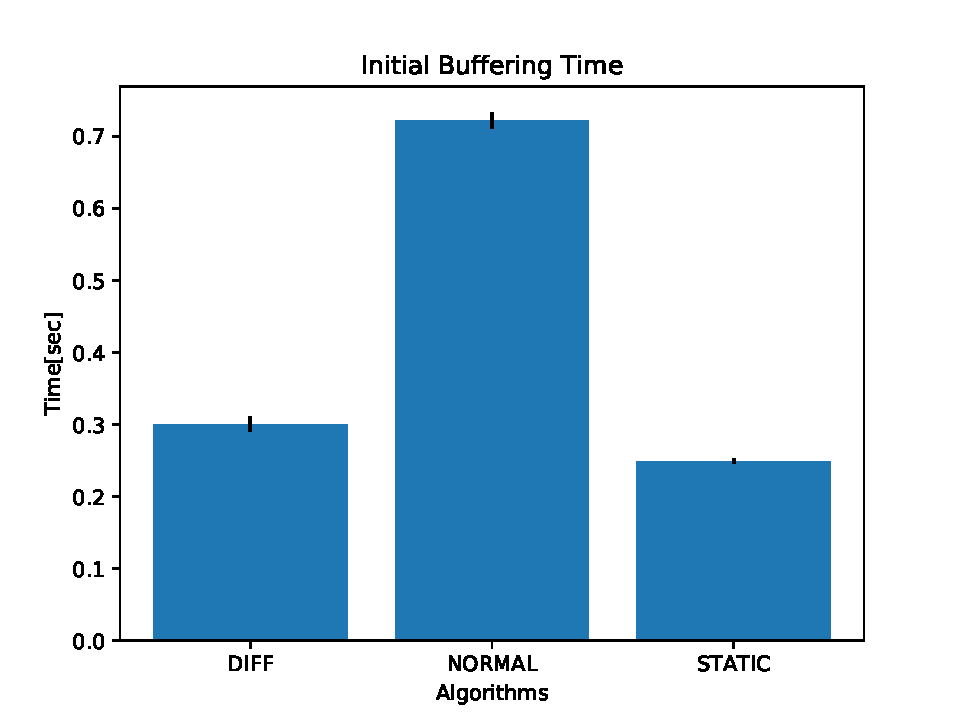
\includegraphics[width=13.5cm]{figure/InitialBufferingTime.pdf}
	\caption{初期バッファリング時間}
	\label{ibt}
\end{figure}

\begin{figure}[h]
	\begin{center}
		\begin{tabular}{cc}
			\begin{minipage}[t]{0.9\hsize}
				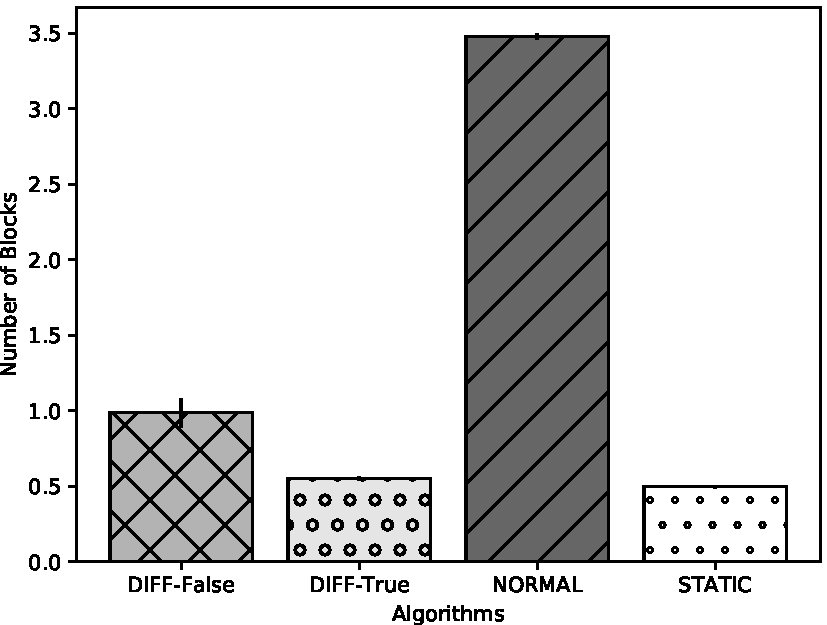
\includegraphics[width=13cm]{figure/NumberofBlocksStayinginBuffer.pdf}
				\caption{平均非有効ブロック数}
				\label{nsb}
			\end{minipage}\\ \\
			\begin{minipage}[t]{0.9\hsize}
				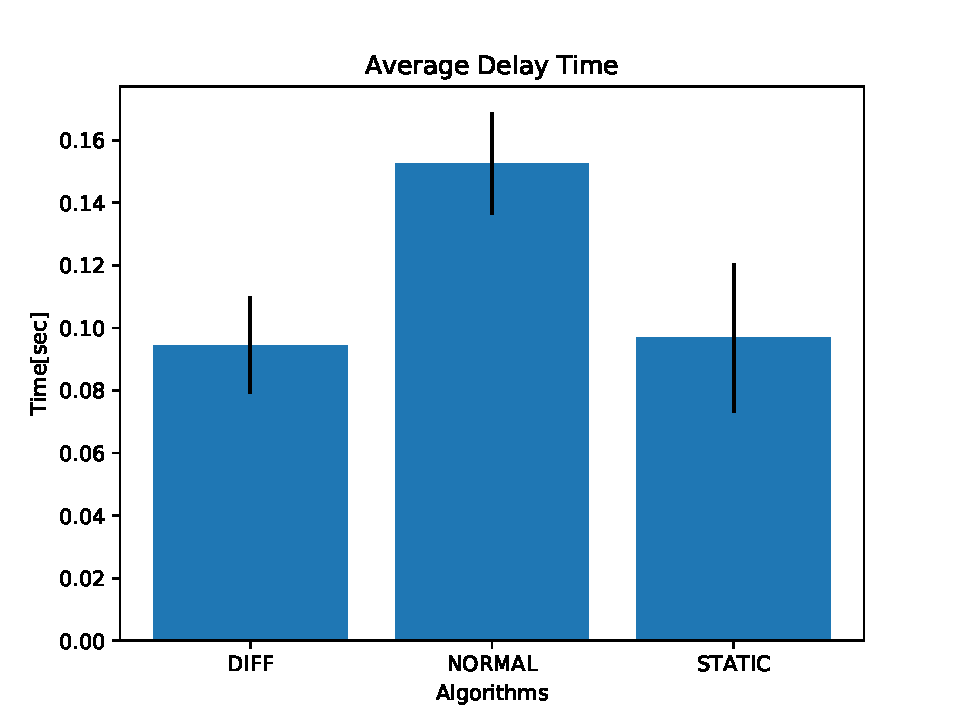
\includegraphics[width=13cm]{figure/AverageDelayTime.pdf}
				\caption{平均遅延時間}
				\label{adt}
			\end{minipage}\\
		\end{tabular}
	\end{center}
\end{figure}

\clearpage

図\ref{ibt}より,初期遅延予測が初期バッファリング時間に与える影響が大きいことが確認できる.
このテストベッドにおける理想的な値である固定遅延要求方式の値に近い値を獲得しており,
また固定遅延要求方式における初期バッファリング時間は,
最も高性能な接続における応答時間とも言い換えることができるので,
理論的に可能な限り初期バッファリング時間を削減していると言える.

図\ref{nsb}より,差分計測を用いた遅延要求方式は非有効ブロック数を大幅に削減することができている.
初期遅延予測を行わない場合は,初期リクエスト時において非有効ブロックが生じていることも確認できる.

図\ref{adt}より,平均遅延時間についても,固定遅延要求方式とほぼ同等の値が得られており,
応答性の向上が確認できる

また,本テストベッド環境のようなネットワーク環境の変化が生じにくい環境では,
遅延要求を行うことで非有効ブロックの発生が抑えられるので,
結果として重複再要求を行うことが殆どないと言える.
よって遅延要求を行うことによる冗長な要求によるネットワーク帯域の使用を減らすことができ,
複数TCP接続を確立することによって得られた帯域を効率的に活用できると言える

\clearpage

\section{公開ネットワークでの評価}
\label{pub}
公開ネットワークでの評価にあたり,Ubuntuのリリースイメージファイルの配布に用いられている公開ミラー\cite{ubuntu}を利用した.
実験には国内2ヶ所,国外7ヶ所の計9ヶ所のミラーを利用した
表\ref{tablemirror}に使用した公開ミラーを示す.
また,参考として各公開ミラーの24時間の性能変化について図\ref{24h}に示す.実験の際にダウンロードしたファイルおよび実験パラメータはテストベッドのものと同一である.
\begin{table}[h]
	\begin{center}
		\caption{使用した公開ミラー一覧}
		\label{tablemirror}
		\begin{tabular}{|l|l|l|} \hline
			ホスト & 組織 & 国\\ \hline \hline
			ftp.jaist.ac.jp & JAIST & JP \\
			ubuntutym2.u-toyama.ac.jp & Univercity of Toyama & JP \\
			releases.ubuntu.com & Canonical & GB \\
			mirrorservice.org & University of Kent & GB \\
			ubuntu.ipacct.com & IPACCT & BG \\
			mirror.pop-sc.rnp.br & PoP-SC & BR \\
			ftp.belnet.be & Belnet & BE \\
			mirrors.mit.edu & MIT & US \\
			mirror.yandex.ru & Yandex & RU \\ \hline
		\end{tabular}
	\end{center}
\end{table}

\begin{figure}[h]
	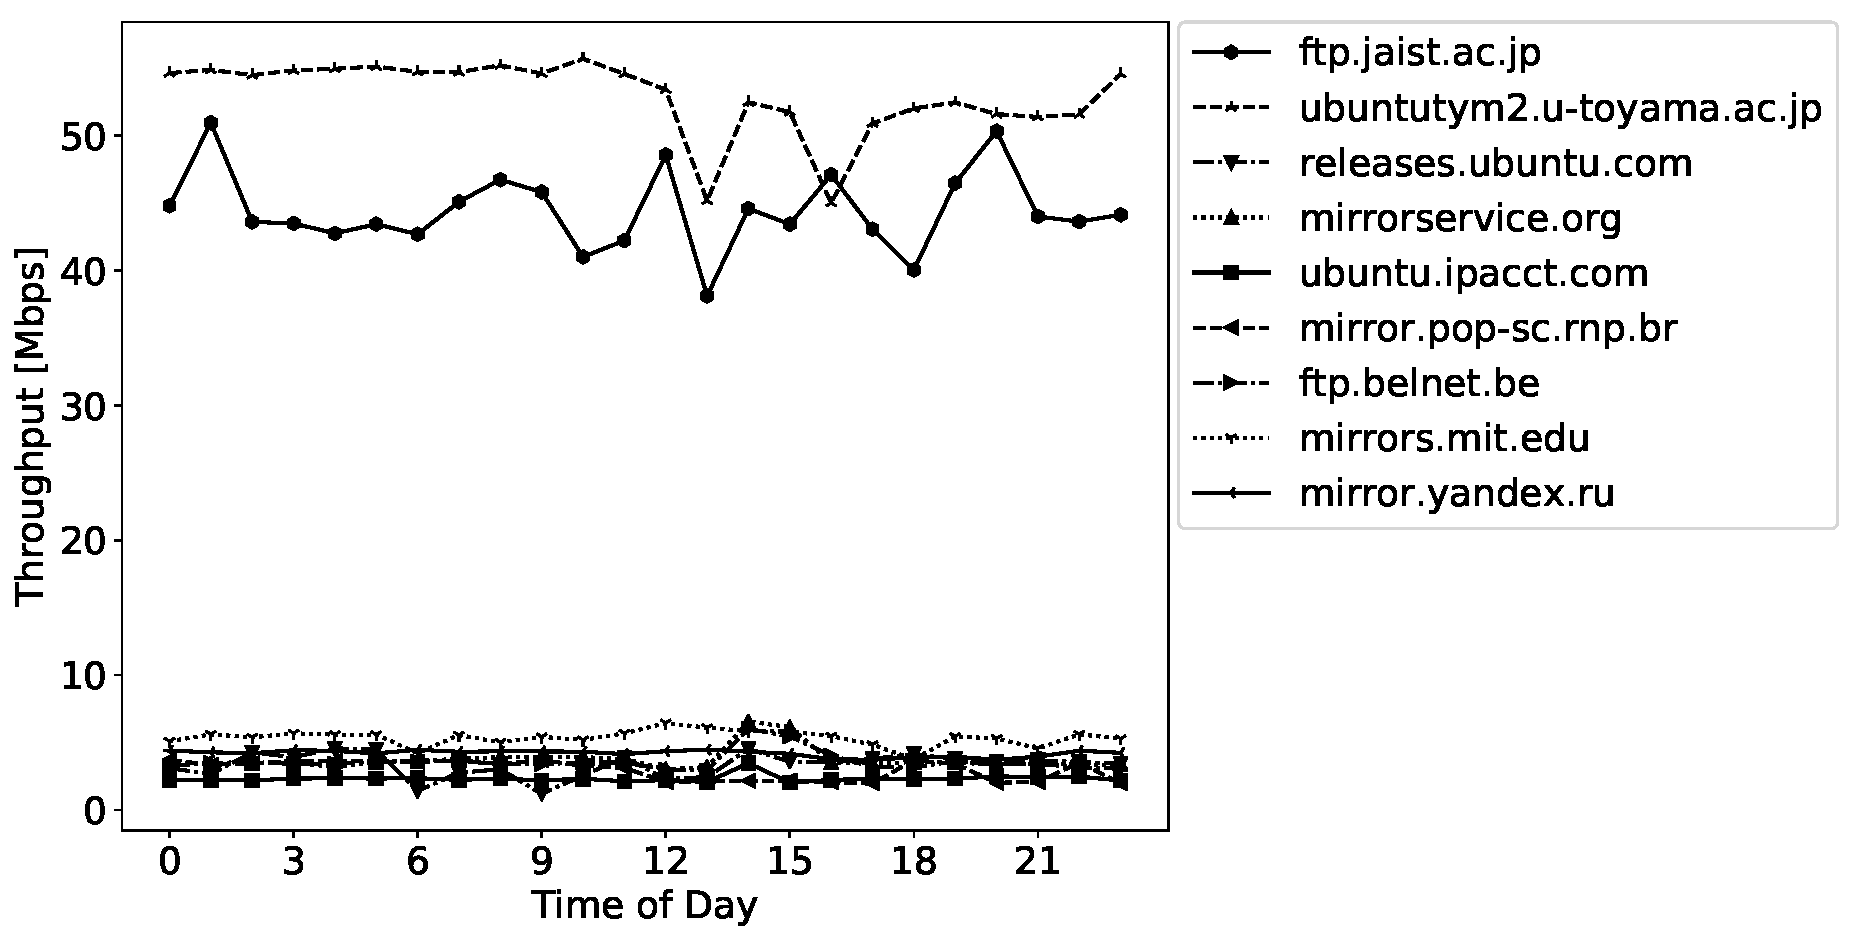
\includegraphics[width=14cm]{figure/thp24h-g.pdf}
	\caption{各公開ミラーの24時間の性能の変化}
	\label{24h}
\end{figure}

\newpage

公開ミラーを利用した実験の結果を図\ref{ibtpub},図\ref{nsbpub}および図\ref{adtpub}に示す.
DIFF-Falseは初期遅延予測を行わない差分計測を用いた遅延要求方式,DIFF-Trueは初期遅延予測を行わない差分計測を用いた遅延要求方式,NORMALは常時最若番を要求する方式(重複再要求のみ),STATICはTCP接続間の性能差を入力する固定遅延要求方式である.
また,10回のすべての試行での各ブロック番号の到着時における非有効ブロック数と遅延時間をプロットしたものを図\ref{allnsb},図\ref{alladt}に示す.
加えて,典型的な受信の様子についてのグラフを図\ref{tpdnpub}および図\ref{tpddpub}に示す.
\begin{figure}[h]
    \begin{tabular}{cc}
       	\begin{minipage}[t]{0.9\hsize}
       		\centering
       		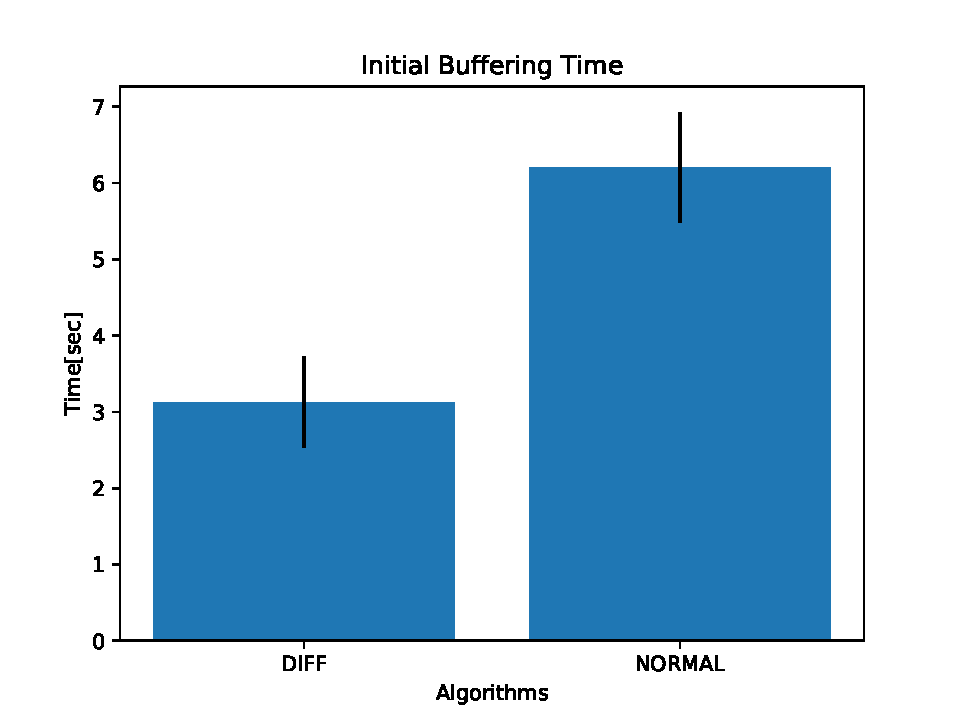
\includegraphics[width=13cm]{figure/InitialBufferingTimePub.pdf}
       		\caption{初期バッファリング時間}
       		\label{ibtpub}
       	\end{minipage}
    \end{tabular}
\end{figure}

\begin{figure}[ht]
		\begin{tabular}{cc}
        	\begin{minipage}[t]{0.9\hsize}
        		\centering
        		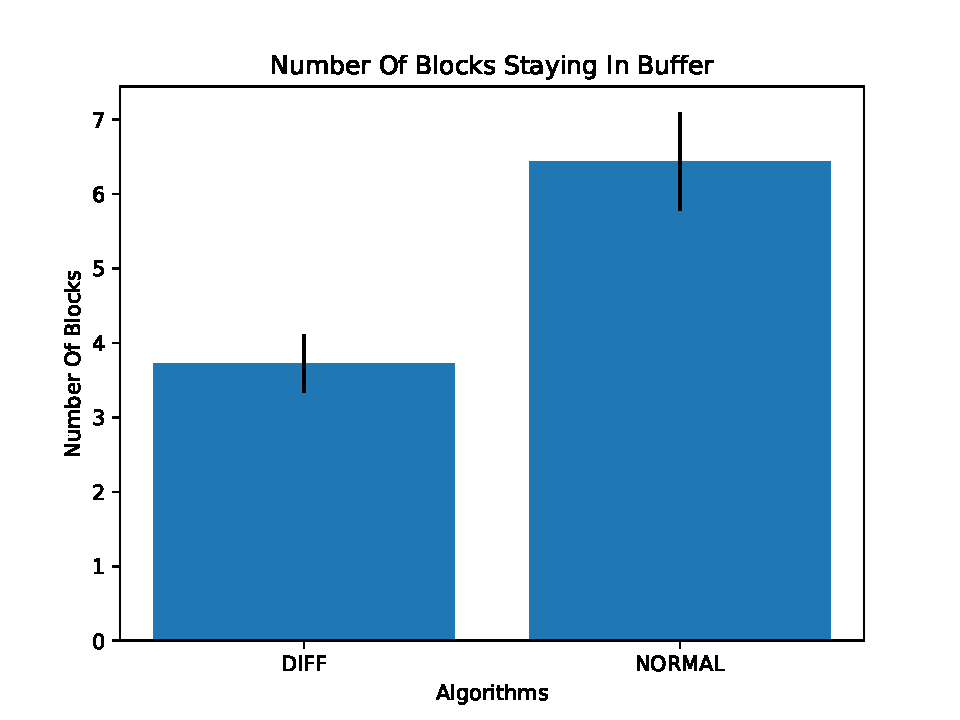
\includegraphics[width=13cm]{figure/NumberOfBlocksStayingInBufferPub.pdf}
        		\caption{平均非有効ブロック数}
        		\label{nsbpub}
        	\end{minipage}\\ \\
			\begin{minipage}[t]{0.9\hsize}
				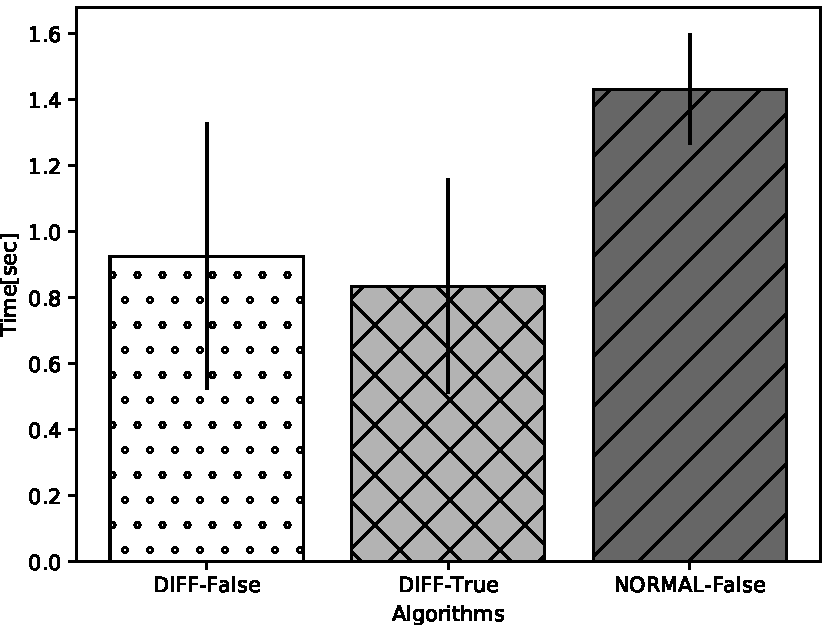
\includegraphics[width=13cm]{figure/AverageDelayTimePub.pdf}
				\caption{平均遅延時間}
				\label{adtpub}
			\end{minipage}
		\end{tabular}
\end{figure}

\clearpage

\begin{figure}[ht]
	\begin{tabular}{cc}
		\begin{minipage}[t]{0.9\hsize}
			\centering
			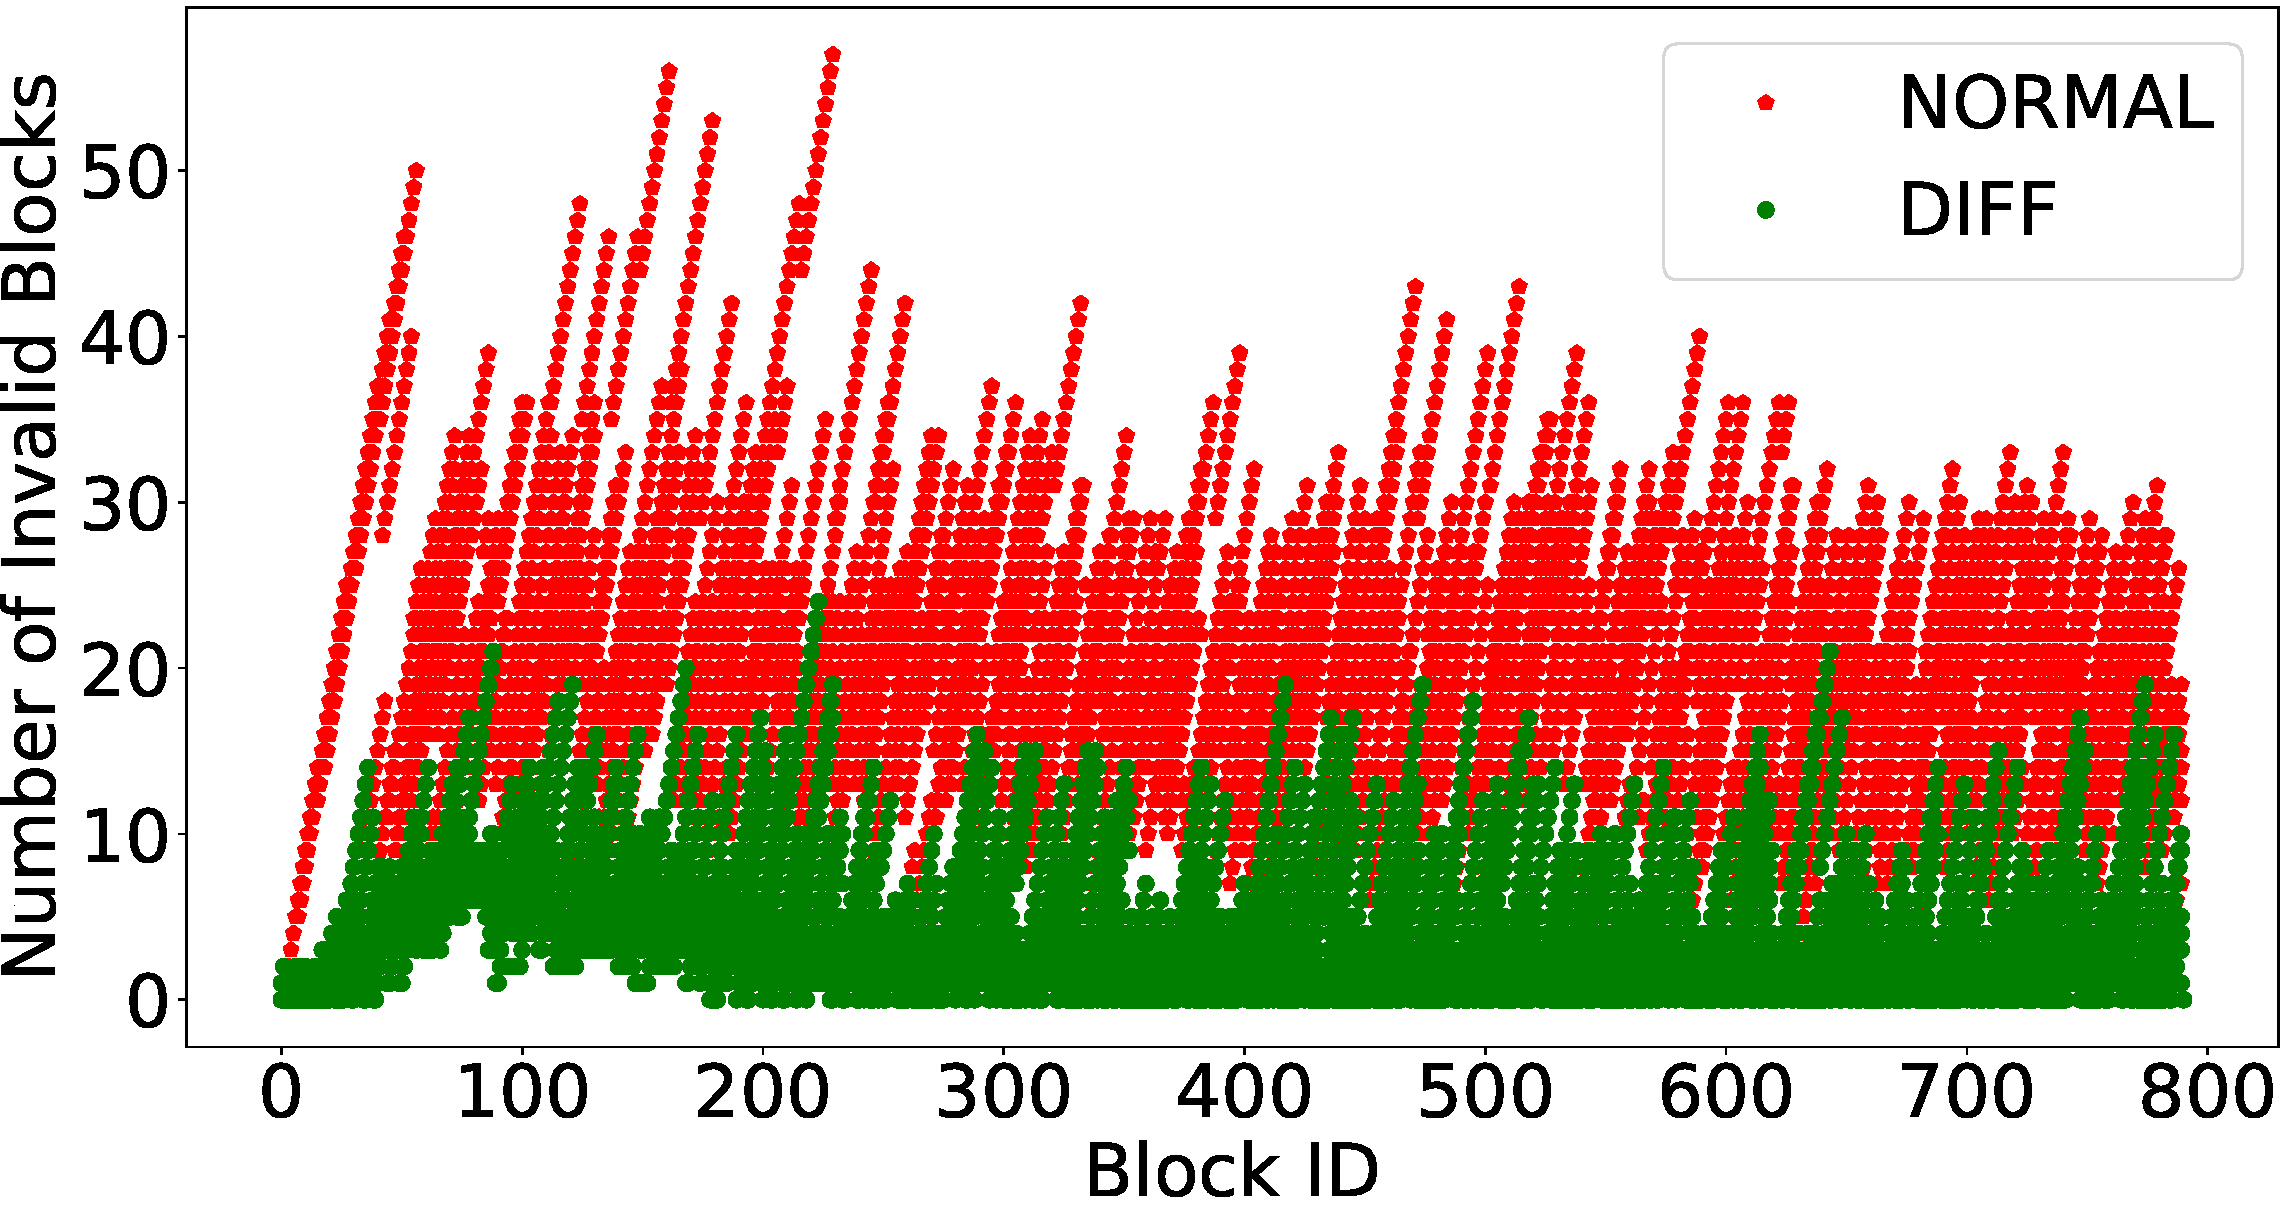
\includegraphics[width=15cm]{figure/allNSB.pdf}
			\caption{非有効ブロック数の分布}
			\label{allnsb}
		\end{minipage}\\ \\ \\
		\begin{minipage}[t]{0.9\hsize}
			\centering
			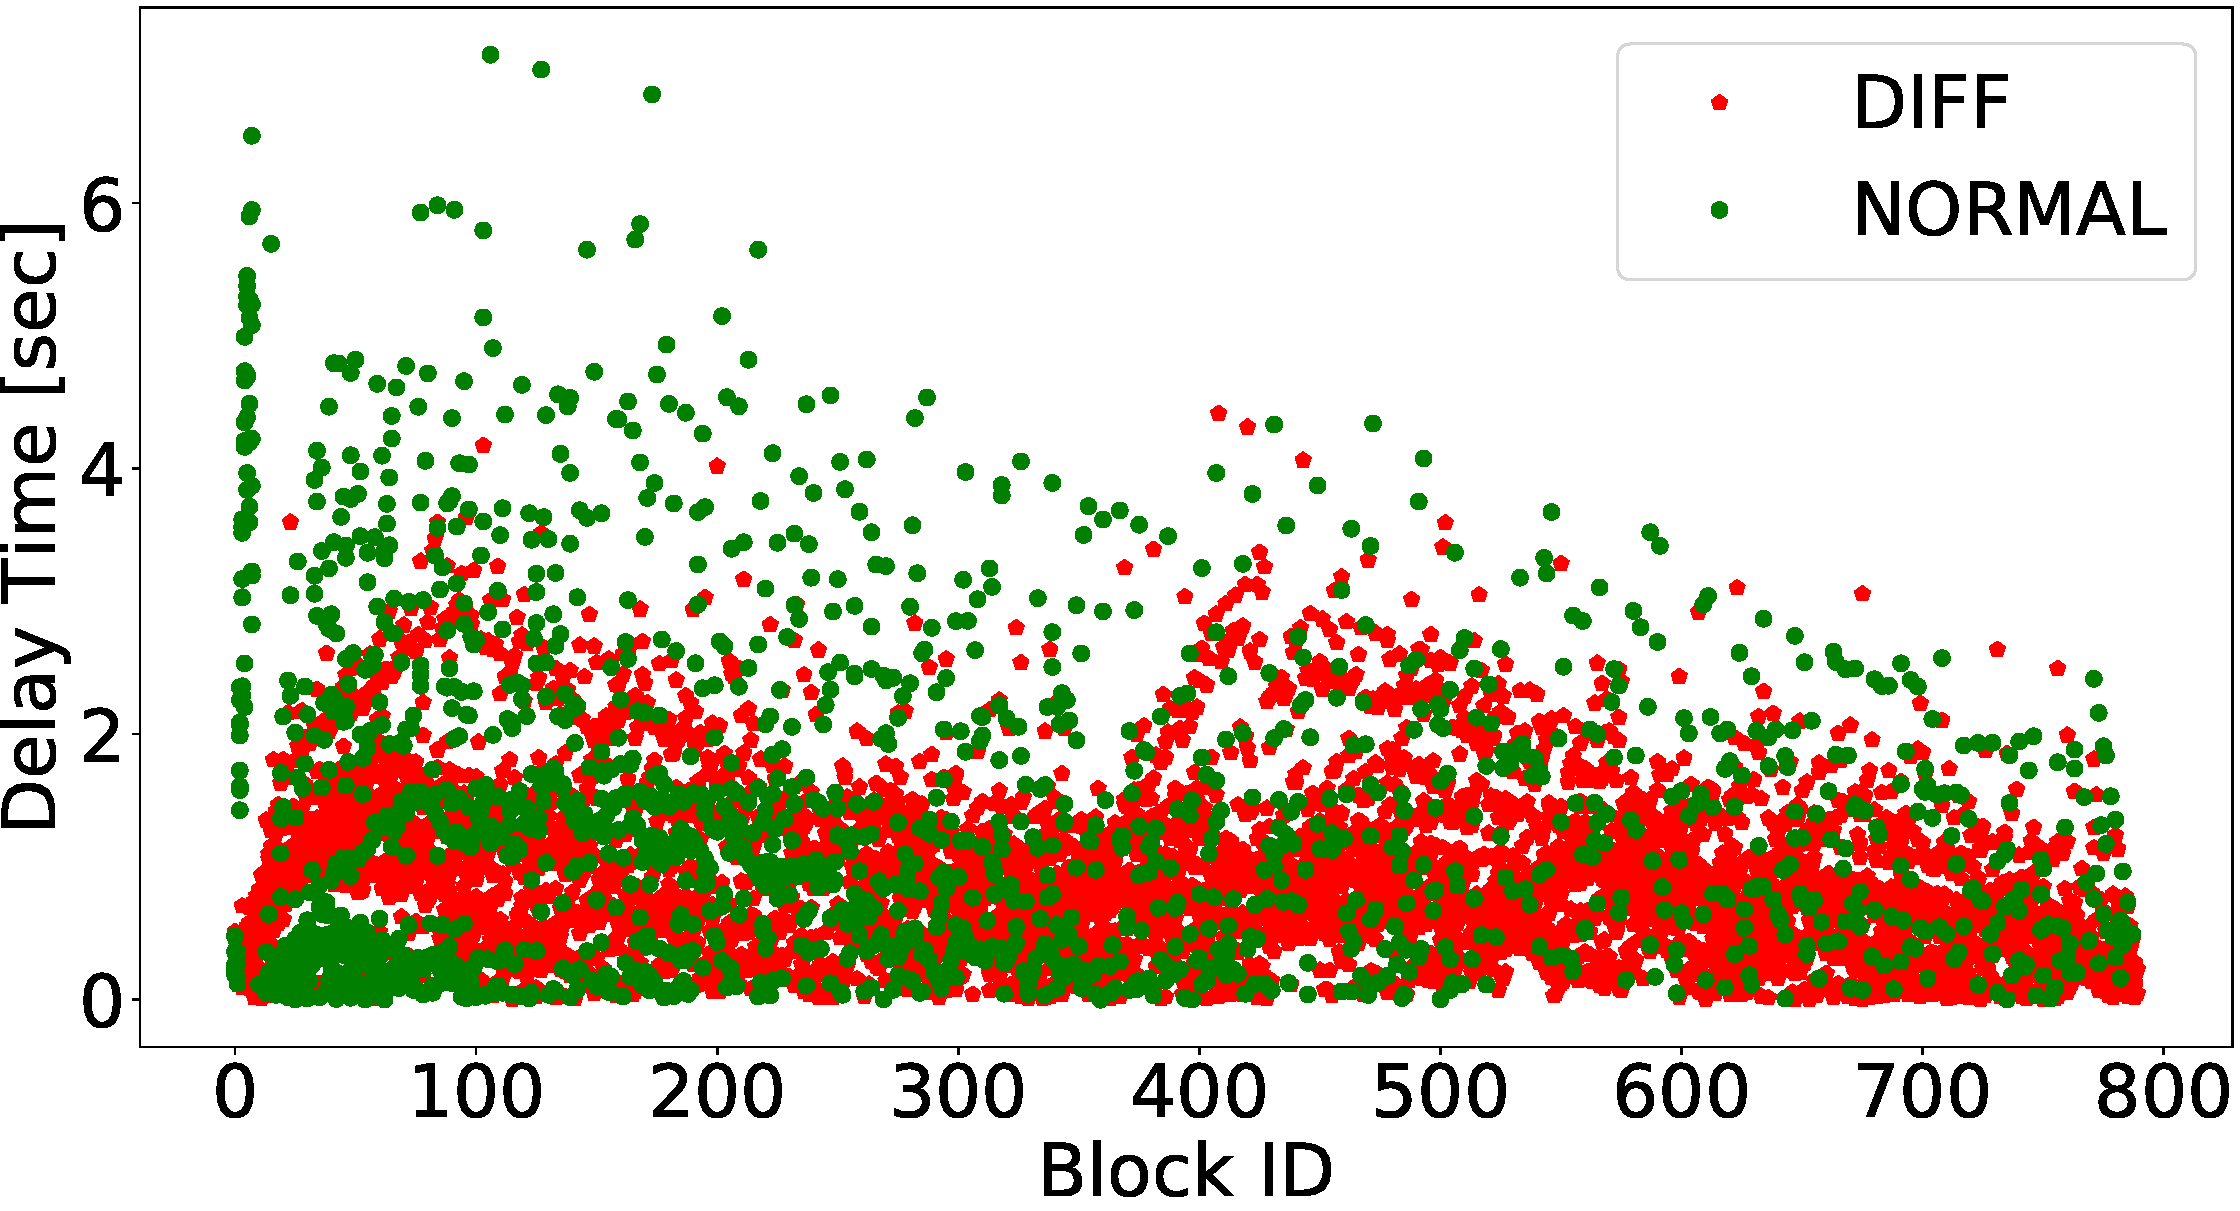
\includegraphics[width=15cm]{figure/allADT.pdf}
			\caption{遅延時間の分布}
			\label{alladt}
		\end{minipage}
	\end{tabular}
\end{figure}

\clearpage

\begin{figure}[ht]
	\begin{tabular}{cc}
		\begin{minipage}[t]{0.9\hsize}
			\centering
			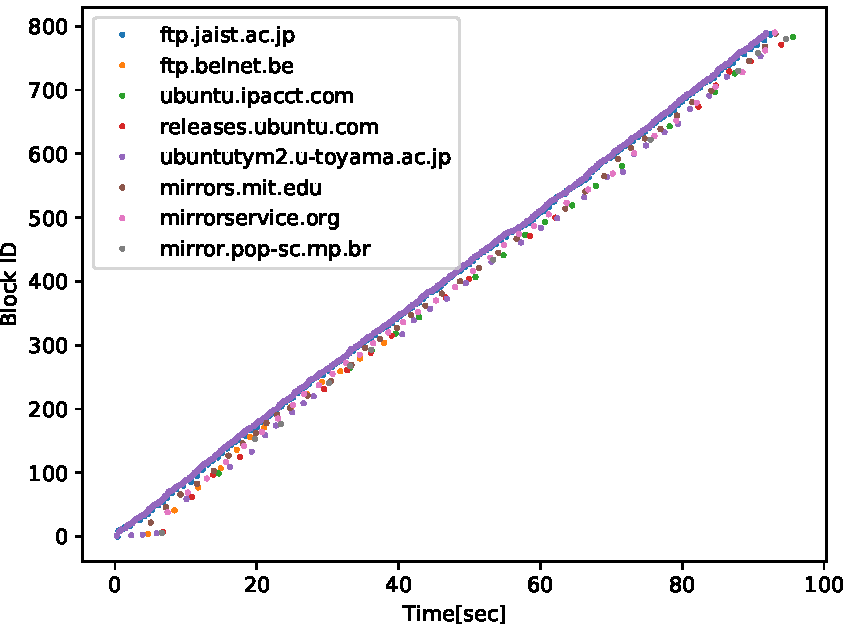
\includegraphics[width=13cm]{figure/TypicalPlotDelay=NORMALInit=FalseDup=IBRC.pdf}
			\caption{遅延要求なしの場合の受信の様子}
			\label{tpdnpub}
		\end{minipage}\\ \\
		\begin{minipage}[t]{0.9\hsize}
			\centering
			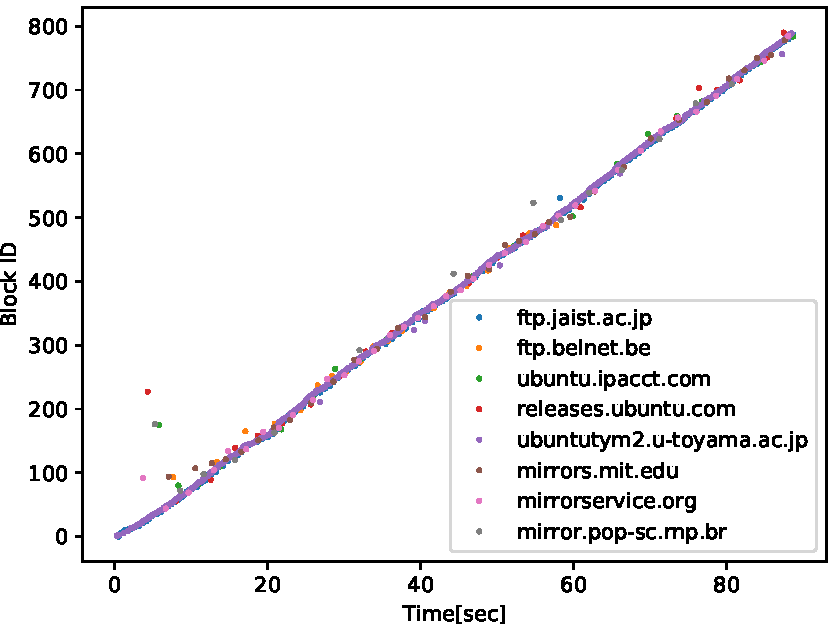
\includegraphics[width=13cm]{figure/TypicalPlotDelay=DIFFInit=TrueDup=IBRC.pdf}
			\caption{差分計測を用いた遅延要求をおこなった場合の受信の様子}
			\label{tpddpub}
		\end{minipage}
	\end{tabular}
\end{figure}

\clearpage

図\ref{ibtpub}〜図\ref{adtpub}より,
提案方式はネットワーク環境についての情報を事前に入力することができない未知の公開ネットワークにおいても,従来方式よりも初期バッファリング時間の削減,非有効ブロック数の削減,平均遅延時間の短縮を確認することができる.
図\ref{ibtpub}より,初期遅延予測を有効にしていない提案方式では初期バッファリング時間がそれほど改善していないことがわかる.
よって初期バッファリング時間には初期のブロックの遅延の影響が大きいことがわかる.
また,図\ref{adtpub}より,平均遅延時間には初期遅延予測の効果はあまりないことがわかる.
なぜなら,初期遅延予測では各接続における最初のブロックの遅延を回避し,
初期バッファリング時間を削減する役割であるための提案であり,
平均遅延時間のような全体的な値への効果は限定的であることがわかる.


図\ref{allnsb}〜図\ref{alladt}より,提案方式では非有効ブロックおよび遅延時間についても値のばらつきが小さいことがわかる.
図\ref{allnsb}がのこぎり型になっているのは,あるブロックが遅延している場合,
そのブロックが到着するまでそのブロックよりも後方のブロックが到着してもそれらのブロックはすべて非有効ブロックとなるからである.
ブロック番号が大きくなるに連れて非有効ブロック数および遅延時間が短くなっているのは,
実装上の都合で,
ある接続において\ref{diff}における\begin{math}D\end{math}の値が最後尾のブロックよりも後ろのブロックを指している場合には,
遅延要求を行わずに接続を解消するという処理を加えているためである.
従来方式の遅延時間が0となっているものが提案方式よりも多いのは,
順序逆転により理想的な到着時刻よりも早く到着してしまったブロックの負の遅延時間はグラフにプロットする際にすべて0として扱っているためである.
非有効ブロック数がブロック番号200近辺まで0にならないのは初期遅延予測において,
実際の性能差以上に後方のブロックを要求した結果,
そのブロックが非有効ブロックとしてバッファ中に滞留し続けているためである.
また,\ref{tpdnpub}における到着時刻の点の集合よりも\ref{tpddpub}における到着時刻の点の集合が,
より細い直線に近づいていることからも,到着順序逆転が減少していることがわかる.
 
%%%%%%%%%%%%%%%%%%%%%%%%%%%%%%%%%%%%%%%%%%%%%%%%%%%%%%%%%%%%%%%%%%%%%%%%%%%%
% 第X章
%%%%%%%%%%%%%%%%%%%%%%%%%%%%%%%%%%%%%%%%%%%%%%%%%%%%%%%%%%%%%%%%%%%%%%%%%%%%%
\chapter{まとめと今後の課題}\label{matomekongo}
本章では,本論文のまとめおよび今後の課題について示す.
\section{まとめ}
本研究ではTCP接続を並列に用いたプログレッシブダウンロードにおいてTCP接続間に性能差が存在する場合に生じる問題点を解消する方式を提案し実装を行った.
提案方式は,各TCP接続におけるブロックの到着間隔を計測することでそのTCP接続に遅延要求を行うことで到着順序の逆転を抑制する方式である.
次に実装したプログラムをテストベッドおよびネットワーク環境が未知の公開ネットワーク上で動作させて評価を行った.
テストベッドでの評価では,差分要求方式はTCP接続間の性能差を入力することなく固定遅延要求方式と同等の性能を獲得することができた.
また,公開ネットワークでの評価では差分計測を用いた遅延予測方式は初期遅延予測方式と組み合わせることで制御なしの場合と比べて,50\%の初期バッファリング時間の削減,50\%の非有効ブロック数の削減と30\%の平均遅延時間の削減が確認できた.


\section{今後の課題}
\hspace*{0.5em}今後の課題として,以下が挙げられる.
\begin{itemize}
    \item 実際のユーザー体験を考慮した評価
    \item タイマ駆動要求方式の実装との比較
    \item 実装の最適化
\end{itemize}

\clearpage
%
%%%%%%%%%%%%%%%%%%%%%%%%%%%%%%%%%%%%%%%%%%%%%%%%%%%%%%%%%%%%%%%%%%%%%%%%%%%%%
% 謝辞
%%%%%%%%%%%%%%%%%%%%%%%%%%%%%%%%%%%%%%%%%%%%%%%%%%%%%%%%%%%%%%%%%%%%%%%%%%%%%
\begin{acknowledgment}
 本研究の機会を与えて頂き,多くの御指導,および御助言を賜わりました
舟阪 淳一 准教授に深甚なる謝意を表します.
また,その他多くの御助言を頂きました諸氏に心より感謝致します.
\end{acknowledgment}
%%%%%%%%%%%%%%%%%%%%%%%%%%%%%%%%%%%%%%%%%%%%%%%%%%%%%%%%%%%%%%%%%%%%%%%%%%%%%
% 参考文献
%%%%%%%%%%%%%%%%%%%%%%%%%%%%%%%%%%%%%%%%%%%%%%%%%%%%%%%%%%%%%%%%%%%%%%%%%%%%%
\begin{flushleft}
\begin {thebibliography}{20} 
	\bibitem{proxy}
	Junichi Funasaka, Atsushi Kawano, and Kenji Ishida: Adaptive Parallel Downloading Method for Proxy Systems, IEICE Trans., Vol.E90-B, No.4, pp.720-727, Apr. 2007.
	
	\bibitem{hiraoka}
	Tokumasa Hiraoka and Junichi Funasaka: A Progressive Download Method Using Multiple TCP Flows on Multiple Paths, Proc. 10th International Conference on Broadband and Wireless Computing, Communication and Applications (BWCCA 2015), pp.318-324, Nov. 2015. 
	
	\bibitem{horiba}
	Hiroaki Horiba, Tokumasa Hiraoka, and Junichi Funasaka: A Progressive Download Method Based on Timer-Driven Requesting Schemes Using Multiple TCP Flows on Multiple Paths, Proc. 37th IEEE ICDCS Workshops, pp.26-31, Jun. 2017.
	
	\bibitem{mhttp}
	Juhoon Kim, Yung-Chih Chen, Ramin Khalili, Don Towsley, Anja Feldmann,
	"Multi-source Multipath HTTP (mHTTP): A Proposal,"
	ACM SIGMETRICS Performance Evaluation Review, vol. 42, No. 1, pp.583--584, 2014.
	
	\bibitem{youtube}
	Youtube.available at https://www.youtube.com,2018.
	
	\bibitem{netflix}
	Netflix.available at https://www.netflix.com,2018.
	
	\bibitem{ubuntu}
	Official CD Mirrors for Ubuntu.available at https://launchpad.net/ubuntu/+cdmirrors, 2018.
	
	\bibitem{vlc}
	VLC.available at https://www.videolan.org/index.html, 2018.
	
	\bibitem{hls}
	Apple Inc., "HTTP Live Streaming (HLS) - Apple Developer", https://developer.apple.com/streaming/
	
	\bibitem{dash}
	ISO org., "ISO/IEC 23009-1:2014 - Information technology -- Dynamic adaptive streaming over HTTP (DASH) -- Part 1: Media presentation description and segment formats", https://www.iso.org/standard/65274.html
\end {thebibliography}
\end{flushleft}

\end{document}
